% \input{mmd6-cpf-leader}
% ***Begin: mmd6-cpf-leader
%
%	Configure LaTeX to produce an article using the memoir class
%

\documentclass[12pt,oneside,oldfontcommands]{memoir}
\usepackage[absolute]{textpos}

% Setup CLARREO Pathfinder document
% \input{mmd6-cpf-setup}
% ***Begin: mmd6-cpf-setup
%
%	Generic Configuration for memoir-based documents
%

\usepackage{layouts}[2001/04/29]

% In case we need a glossary, or index
\usepackage[automake,acronyms,shortcuts,nopostdot,nonumberlist,nogroupskip]{glossaries}
\renewcommand{\glossarysection}[2][]{}
\setglossarystyle{longheader}
\renewcommand{\entryname}{Acronym}
\renewcommand{\descriptionname}{Complete Term}
\setlength{\glsdescwidth}{1\linewidth}
\glstoctrue
\makeglossaries
\makeindex

% Basic page layout configuration
\def\mychapterstyle{default}
\def\mypagestyle{headings}










% ***End: mmd6-cpf-setup

% Use 8.5 x 11 inch page layout
% \input{mmd6-cpf-layout-8.5x11}
% ***Begin: mmd6-cpf-layout-8.5x11
%
%	8.5 x 11 layout for CPF memoir-based documents
%


%%% need more space for ToC page numbers
\setpnumwidth{1.0em}
\setrmarg{3.55em}

%%% need more space for ToC section numbers
\cftsetindents{part}{0.5em}{3em}
\cftsetindents{chapter}{1.0em}{3em}
\cftsetindents{section}{3.0em}{4.25em}
\cftsetindents{subsection}{4.25em}{3.0em}
\cftsetindents{subsubsection}{8.4em}{4.8em}
\cftsetindents{paragraph}{10.7em}{5.7em}
\cftsetindents{subparagraph}{12.7em}{6.7em}

%%% need more space for LoF numbers
\cftsetindents{figure}{1.0em}{3.0em}

%%% and do the same for the LoT
\cftsetindents{table}{1.0em}{3.0em}

%%% set up the page layout
\settrimmedsize{\stockheight}{\stockwidth}{*}	% Use entire page
\settrims{0pt}{0pt}

\setlrmarginsandblock{1.5in}{1.5in}{*}
\setulmarginsandblock{1.5in}{1.5in}{*}
\setmarginnotes{17pt}{51pt}{\onelineskip}
\setheadfoot{2\onelineskip}{.4\onelineskip}
\setheaderspaces{*}{2\onelineskip}{*}
\checkandfixthelayout% ***End: mmd6-cpf-layout-8.5x11

% Use default packages for memoir, cdh, and CPF setup
% \input{mmd6-memoir-packages}
% ***Begin: mmd6-memoir-packages
%
%	Default packages for memoir documents created by MultiMarkdown
%

\usepackage{fancyvrb}			% Allow \verbatim et al. in footnotes
\usepackage{graphicx}			% To enable including graphics in pdf's
\usepackage{booktabs}			% Better tables
\usepackage{tabulary}			% Support longer table cells
\usepackage[T1]{fontenc}		% Use T1 font encoding for accented characters
\usepackage[utf8]{inputenc}		% For UTF-8 support
\usepackage{xcolor}				% Allow for color (annotations)
\usepackage{listings}			% Allow for source code highlighting
\usepackage[sort&compress]{natbib} % Better bibliography support

% \usepackage[normalem]{ulem}		% Support strikethrough

% \input{mmd6-criticmarkup}
% ***Begin: mmd6-criticmarkup
% CriticMarkup Support
\usepackage{soul}
\usepackage{xargs}
\usepackage{todonotes}
\newcommandx{\cmnote}[2][1=]{\todo[linecolor=red,backgroundcolor=red!25,bordercolor=red,#1]{#2}}

% ***End: mmd6-criticmarkup
% ***End: mmd6-memoir-packages
% \input{mmd6-cdh-packages}
% ***Begin: mmd6-cdh-packages
\let\footruleskip\undefined %undefine footruleskip

\usepackage{fancyhdr}
\usepackage{amsmath}
\usepackage{amssymb}
\usepackage[version=3]{mhchem}
\usepackage{lastpage}
\usepackage{mathabx}
\usepackage{mathrsfs}
\usepackage[margin=1.0in]{geometry}
\usepackage{siunitx}
\usepackage{enumitem}
\usepackage{lineno}
\usepackage{placeins}
\usepackage{pdflscape}
\usepackage{placeins}
\usepackage[normalem]{ulem}
\usepackage{ebgaramond}
\usepackage{longtable}
\usepackage{multicol}
\usepackage{microtype}
\usepackage{etoolbox}
\usepackage{footmisc}
\usepackage{fontspec}
\setsansfont{Helvetica}
\setmainfont{Times New Roman}
% \defaultfontfeatures{Ligatures=TeX}
% \setmainfont{EB Garamond}
% \fontspec[ItalicFont={EB Garamond 12 Italic}]
% \setmonofont{Inconsolata}
% \setmathsfont(Digits,Latin,Greek){TeX Gyre Termes}
% \renewcommand\emshape{\itshape}

% \usepackage{acronym}
% \usepackage{mathspec}
% \usepackage{caption}
% \usepackage{lscape}
% \usepackage[titletoc]{appendix}
% \usepackage[perpage,symbol*]{footmisc}
% \usepackage[symbol*]{footmisc}
% \usepackage{layouts}
% \usepackage{cleveref}
% \let\printglossary\relax
% \let\theglossary\relax
% \let\endtheglossary\relax
% \def\bibliostyle{chicago}
% \usepackage{wasysym}




% ***End: mmd6-cdh-packages
% \input{mmd6-cpf-packages}
% ***Begin: mmd6-cpf-packages
\usepackage[para,flushleft]{threeparttable}% ***End: mmd6-cpf-packages

% Configure default metadata to avoid errors
% \input{mmd6-default-metadata}
% ***Begin: mmd6-default-metadata
%
%	Configure default metadata in case it's missing to avoid errors
%

\def\myauthor{Author}
\def\defaultemail{}
\def\defaultposition{}
\def\defaultdepartment{}
\def\defaultaddress{}
\def\defaultphone{}
\def\defaultfax{}
\def\defaultweb{}
\def\defaultaffiliation{}

\def\mytitle{Title}
\def\subtitle{}
\def\mykeywords{}
% \def\keywords{}


\def\bibliostyle{plain}
% \def\bibliocommand{}

\def\myrecipient{}

% Overwrite with your own if desired
%\input{ftp-metadata}

% ***End: mmd6-default-metadata

% \input{mmd6-cpf-header-reformat}
% ***Begin: mmd6-cpf-header-reformat

%

% %
% % Define Page Styles
% %
% \pagestyle{fancy}
% \setlength\hoffset{-0.2in}
% \setlength\topmargin{-20pt}
% \setlength\textheight{600pt}
% \setlength\footskip{50pt}
% \renewcommand{\headrulewidth}{0.0pt}
% % Hard-coded title due to mutlicolumn error
% \lhead{\begin{tabular}[b]{|p{3.75in}|p{2.7in}|} \hline Revision:~\revision & Document No:~\documentnumber\\ \hline Release Date:~\releasedate&Page:~\thepage~of~\pageref{LastPage}\\ \hline \multicolumn{2}{|l|}{Title:~Mission Concept of Operations}\\ \hline \end{tabular}}
% % \lhead{\begin{tabular}[b]{|p{3.75in}|p{2.7in}|} \hline Revision:~\revision & Document No:~\documentnumber\\ \hline Release Date:~\releasedate&Page:~\thepage~of~\pageref{LastPage}\\ \hline \multicolumn{2}{|l|}{Title:~\mytitle}\\ \hline \end{tabular}}
% \chead{}
% % \chead{\mytitle}
% \rhead{}
% \cfoot{\scriptsize The electronic version is the offical approved document.\\Verify this is the correct version before use.}


% \fancypagestyle{firststyle}
% {
%    \fancyhf{}
%    \fancyfoot[C]{\scriptsize  The electronic version is the offical approved document.\\Verify this is the correct version before use.}
%    \setlength\topmargin{-40pt}
%    \setlength\footskip{-65pt}
% }
% %
% % End Define Page Styles
% %
% % CPF SMRD-specific page styles to enable compile-time modification of revision and footer
%
% Define Page Styles
%
\pagestyle{fancy}
\setlength\hoffset{-0.2in}
\setlength\topmargin{-20pt}
\setlength\textheight{600pt}
\setlength\footskip{50pt}
\renewcommand{\headrulewidth}{0.0pt}
% Hard-coded title due to mutlicolumn error
\lhead{\begin{tabular}[b]{|p{3.75in}|p{2.7in}|} \hline Revision:~\revision & Document No:~\documentnumber\\ \hline Release Date:~\releasedate&Page:~\thepage~of~\pageref{LastPage}\\ \hline \multicolumn{2}{|l|}{Title:~Science and Mission Requirements Document}\\ \hline \end{tabular}}
\chead{}
% \chead{\mytitle}
\rhead{}
\cfoot{\scriptsize The electronic version is the official approved document.\\The requirements are from a CORE database query dated: 13 April 2018.\\Verify this is the correct version before use.}


\fancypagestyle{firststyle}
{
   \fancyhf{}
   \fancyfoot[C]{\scriptsize  The electronic version is the official approved document.\\The requirements are from a CORE database query dated: 13 April 2018.\\Verify this is the correct version before use.}
   \setlength\topmargin{-40pt}
   \setlength\footskip{-65pt}
}
%
% End Define Page Styles
%

% ***Begin: mmd6-cpf-page-styles
%
% Define Page Styles
%
\pagestyle{fancy}
\setlength\hoffset{-0.2in}
\setlength\topmargin{-20pt}
\setlength\textheight{600pt}
\setlength\footskip{50pt}
\renewcommand{\headrulewidth}{0.0pt}
% Hard-coded title due to mutlicolumn error
\lhead{\begin{tabular}[b]{|p{3.75in}|p{2.7in}|} \hline Revision:~\revision & Document No:~\documentnumber\\ \hline Release Date:~\releasedate&Page:~\thepage~of~\pageref{LastPage}\\ \hline \multicolumn{2}{|l|}{Title:~Mission Concept of Operations}\\ \hline \end{tabular}}
\chead{}
% \chead{\mytitle}
\rhead{}
\cfoot{\scriptsize The electronic version is the official approved document.\\Verify this is the correct version before use.}


\fancypagestyle{firststyle}
{
   \fancyhf{}
   \fancyfoot[C]{\scriptsize  The electronic version is the official approved document.\\Verify this is the correct version before use.}
   \setlength\topmargin{-40pt}
   \setlength\footskip{-65pt}
}
%
% End Define Page Styles
%% ***End: mmd6-cpf-page-styles

% New Capitalize Macro
\makeatletter
\newcommand{\Capitalize}[1]{%
  \edef\@tempa{\expandafter\@gobble\string#1}%
  \edef\@tempb{\expandafter\@car\@tempa\@nil}%
  \edef\@tempa{\expandafter\@cdr\@tempa\@nil}%
  \uppercase\expandafter{\expandafter\def\expandafter\@tempb\expandafter{\@tempb}}%
  \@namedef{\@tempb\@tempa}{\expandafter\MakeUppercase\expandafter{#1}}}
\makeatother
% End New Capitalize Macro


\makeatletter
\let\ps@plain\ps@fancy
\makeatother

% Formatting of TOC

%
% Redefine document section hyperref labels
%
\def\subsubsectionautorefname{Section}
\def\subsectionautorefname{Section}
\def\sectionautorefname{Section}
\def\chapterautorefname{Section}
%
% Complete hyperref label redefinition
%

% \tightlists
\setlist{itemsep=.1mm, topsep=0mm}
\setlist[enumerate,1]{leftmargin=0.5cm}
\renewcommand{\theenumi}{\alph{enumi}}

% \renewcommand*{\afterlottitle}{\vspace{0em}}


%
% Define Chapter Styles
%
\makechapterstyle{cpf}{%
\setlength{\afterchapskip}{-0.5\baselineskip}
  \setlength{\beforechapskip}{\baselineskip}
  \setlength{\headsep}{2.0\baselineskip}
  \renewcommand*{\chapterheadstart}{}
  \renewcommand*{\printchaptername}{}
  \renewcommand*{\chapternamenum}{}
  \renewcommand*{\printchapternum}{\sffamily\large\bfseries\thechapter.0\space}
  \renewcommand*{\afterchapternum}{}
  \renewcommand{\printchaptertitle}[1]{%
    \raggedright{##1}}
}

\makechapterstyle{appendix}{%
  \setlength{\afterchapskip}{\baselineskip}
  \setlength{\beforechapskip}{\baselineskip}
  \setlength{\headsep}{2.0\baselineskip}
  \renewcommand*{\chapterheadstart}{}
  \renewcommand*{\printchaptername}{\sffamily\large\center\bfseries APPENDIX\space}
  \renewcommand*{\chapternamenum}{}
  \renewcommand*{\printchapternum}{\thechapter\space}
  \renewcommand*{\afterchapternum}{}
  \renewcommand{\printchaptertitle}[1]{%
    \center\bfseries{##1}}
}
%
% End Chapter Styles Definition
%

%
% Define Table Styles to enable bold first row
%
\newcolumntype{+}{>{\global\let\currentrowstyle\relax}}
\newcolumntype{^}{>{\currentrowstyle}}
\newcommand{\rowstyle}[1]{\gdef\currentrowstyle{#1}%
#1\ignorespaces
}
%
% End Table Style Definition
%


%
%
% Define Table of Contents, Figures, Tables, Appendices Formatting
%
\renewcommand{\contentsname}{\large\sffamily TABLE OF CONTENTS}
\renewcommand{\listfigurename}{\large\sffamily TABLE OF FIGURES}
\renewcommand{\cftfigurename}{Figure\space}
\renewcommand{\listtablename}{\large\sffamily TABLE OF TABLES}
\renewcommand{\cfttablename}{Table\space}
\renewcommand{\cftappendixname}{\normalsize Appendix\space}
\renewcommand{\cftchapteraftersnum}{.0}
\renewcommand{\cftchapterfont}{\normalfont}
\renewcommand{\cftchapterpagefont}{\normalfont}
\renewcommand{\cftsectionfont}{\normalsize}
\setlength{\cftbeforechapterskip}{0.0in}
\renewcommand{\cftchapterdotsep}{\cftdotsep}% Chapters should use dots in ToC
\renewcommand{\printtoctitle}[1]{\centering\Large\bfseries #1}
\renewcommand{\printloftitle}[1]{\centering\Large\bfseries #1}
\renewcommand{\printlottitle}[1]{\centering\Large\bfseries #1}
\renewcommand{\aftertoctitle}{%
	\par\nobreak\normalsize\bfseries\quad SECTION\mbox{}\hfill{PAGE}\par\nobreak}
\renewcommand{\afterlottitle}{%
	\par\nobreak}
\renewcommand{\afterloftitle}{%
	\par\nobreak}
\setcounter{tocdepth}{2}
% End Table of Contents, Figures, Tables, Appendices Formatting


%
% Define Table of Appendices
%
\cftinsertcode{preapp}{\setcounter{tocdepth}{-10}}
\newcommand\apptoc{
  \begingroup
  \cftinsertcode{prenorm}{\setcounter{tocdepth}{-10}}
  \cftinsertcode{preapp}{\setcounter{tocdepth}{0}}
  \renewcommand\contentsname{\large\sffamily TABLE OF APPENDICES}
  \renewcommand{\aftertoctitle}{\par}
  \renewcommand{\cftchapteraftersnum}{}
  \normalfamily
  \tableofcontents*
 \endgroup
}
%
% End Table of Appendices Definitions
%


%
% Section Heading Formatting
%
\makeatletter
\renewcommand\paragraph{\@startsection
 {paragraph}{4}{0mm}%
 {-\baselineskip}%
 {1.0\baselineskip}%
 {\sffamily\bfseries\normalsize}}%
\makeatother

\makeatletter
\renewcommand\subparagraph{\@startsection
 {subparagraph}{5}{0mm}%
 {-\baselineskip}%
 {1.0\baselineskip}%
 {\sffamily\bfseries\normalsize}}%
\makeatother

\setsecheadstyle{\bfseries\sffamily\raggedright}
\setsubsecheadstyle{\bfseries\sffamily\raggedright}
\setsubsubsecheadstyle{\bfseries\sffamily\raggedright}

%
% End Section Heading Formatting
%

\makeatletter
\let\ps@plain\ps@fancy
\makeatother
% ***End: mmd6-cpf-header-reformat
% ***End: mmd6-cpf-leader
\def\myauthor{Craig Hutchinson}
\def\mytitle{Power Converter Unit Interface Control Document}
\def\mydate{17 April 2018}
\def\releasedate{TBD}
\def\documentnumber{CPF-02-024}
\def\titlepagerevision{PRELIMINARY}
\def\revision{Preliminary  }
\def\watermark{Draft}
\newacronym{ABI}{ABI}{Advanced Baseline Imager}

\newacronym{ADCO}{ADCO}{Attitude Determination and Control Officer}

\newacronym{AFRAM}{AFRAM}{Active Flight Releasable Attachment Mechanism}

\newacronym{AGRI}{AGRI}{Advanced Geosynchronous Radiation Imager}

\newacronym{ASDC}{ASDC}{Atmospheric Sciences Data Center}

\newacronym{ATBD}{ATBD}{Algorithm Theoretical Basis Document}

\newacronym{ATL}{ATL}{Attitude Timeline}

\newacronym{AVHRR}{AVHRR}{Advanced Very High Resolution Radiometer}

\newacronym{BAD}{BAD}{Broadcast Ancillary Data}

\newacronym{BASEPLATE}{BASEPLATE}{Beta, Attitude, Significant Event Planning Table}

\newacronym{CERES}{CERES}{Clouds and Earth's Radiant Energy System}

\newacronym{CLARREO}{CLARREO}{Climate Absolute Radiance and Refractivity Observatory}

\newacronym{COMS}{COMS}{Communication, Ocean, and Meteorological Satellite}

\newacronym{CPF}{CPF}{CLARREO Pathfinder}

\newacronym{CPOC}{CPOC}{CPF Payload Operations Center}

\newacronym{CPRSP}{CPRSP}{CLARREO Pathfinder Reflected Solar Payload}

\newacronym{CSDS}{CSDS}{CPF Science Data System}

\newacronym{CSTOL}{CSTOL}{Colorado System Test and Operations Language}

\newacronym{DAAC}{DAAC}{Distributed Active Archive Center}

\newacronym{DEWG}{DEWG}{Dynamic Events Working Group}

\newacronym{EE}{EE}{Electrical Engineer}

\newacronym{EOSDIS}{EOSDIS}{Earth Observing System Data and Information System}

\newacronym{ESDIS}{ESDIS}{Earth Science Data and Information System}

\newacronym{ELC}{ELC}{ExPRESS Logistics Carrier}

\newacronym{EOTP}{EOTP}{Enhanced ORU Temporary Platform}

\newacronym{EUMETSAT}{EUMETSAT}{European Organization for the Exploitation of Meteorological Satellites}

\newacronym{ExPA}{ExPA}{ExPRESS Pallet Adapter}

\newacronym{ExPRESS}{ExPRESS}{Expedite the Processing of Experiments to Space Station}

\newacronym{FC}{FC}{Flight Controller}

\newacronym{FD}{FD}{Flight Director}

\newacronym{FLAWS}{FLAWS}{Flight Anomaly Worksheet}

\newacronym{FPA}{FPA}{Focal Plane Array}

\newacronym{FPE}{FPE}{Focal Plane Electronics}

\newacronym{FOV}{FOV}{Field of View}

\newacronym{FRAM}{FRAM}{Flight Releasable Attach Mechanism}

\newacronym{FSW}{FSW}{Flight Software}

\newacronym{GEO}{GEO}{Geostationary Earth Orbit}

\newacronym{GOCI}{GOCI}{Geostationary Ocean Color Imager}

\newacronym{GOES}{GOES}{Geostationary Operational Environmental Satellite}

\newacronym{GRAWS}{GRAWS}{Ground Anomaly Worksheet}

\newacronym{GSFC}{GSFC}{Goddard Space Flight Center}

\newacronym{HFSS}{HFSS}{High-rate Fine Sun Sensor}

\newacronym{HOSC}{HOSC}{Huntsville Operations Support Center}

\newacronym{H&S}{H&S}{Health and Status}

\newacronym{HySICS}{HySICS}{HyperSpectral Imager for Climate Science}

\newacronym{HPS}{HPS}{HySICS Pointing System}

\newacronym{HVPS}{HVPS}{High Voltage Power Supply}

\newacronym{IC SIPS}{IC SIPS}{Inter-Calibration Science Investigator Processing System}

\newacronym{ICPP}{ICPP}{Inter-Calibration Planning and Processing element}

\newacronym{ICS}{ICS}{ISS Communications Services}

\newacronym{IT}{IT}{Information Technology}

\newacronym{IMU}{IMU}{Inertial Measurement Unit}

\newacronym{IRS}{IRS}{Indian Remote Sensing}

\newacronym{HISIE}{HISIE}{HySICS Instrument-Spacecraft Interface Electronics}

\newacronym{ICD}{ICD}{Interface Control Document}

\newacronym{IDD}{IDD}{Interface Definition Document}

\newacronym{ISRO}{ISRO}{Indian Space Research Organization}

\newacronym{ISS}{ISS}{International Space Station}

\newacronym{JPSS}{JPSS}{Joint Polar Satellite System}

\newacronym{JSC}{JSC}{Johnson Space Center}

\newacronym{KARI}{KARI}{Korea Aerospace Research Institute}

\newacronym{KSC}{KSC}{Kennedy Space Center}

\newacronym{LAADS}{LAADS}{Level-1 and Atmosphere Archive and Distribution System}

\newacronym{LaRC}{LaRC}{Langley Research Center}

\newacronym{LASP}{LASP}{The University of Colorado Laboratory for Atmospheric and Space Physics}

\newacronym{LEO}{LEO}{Low Earth Orbit}

\newacronym{LPF}{LPF}{Launch Provider Facility}

\newacronym{MCC-H}{MCC-H}{Mission Control Center-Houston}

\newacronym{MODS}{MODS}{Mission Operations and Data Systems}

\newacronym{MSFC}{MSFC}{Marshall Space Flight Center}

\newacronym{MTG-I}{MTG-I}{Meteosat Third Generation-Imaging}

\newacronym{NATC}{NATC}{NASA Threaded Coupling}

\newacronym{NOAA}{NOAA}{National Oceanic and Atmospheric Administration}

\newacronym{NPP}{NPP}{National Polar-orbiting Partnership}

\newacronym{OASIS-CC}{OASIS-CC}{Operations and Science Instrument Support Command Control}

\newacronym{OASIS-PS}{OASIS-PS}{Operations and Science Instrument Support Planning and Scheduling}

\newacronym{OLI}{OLI}{Operational Land Imager}

\newacronym{ORU}{ORU}{Orbital Replacement Unit}

\newacronym{OTCM}{OTCM}{ORU Tool Changeout Mechanism}

\newacronym{PCU}{PCU}{Power Converter Unit}

\newacronym{PDL}{PDL}{Payload Data Library}

\newacronym{PFRAM}{PFRAM}{Passive Flight Releasable Attachment Mechanism}

\newacronym{POIC}{POIC}{Payload Operations Integration Center}

\newacronym{PRCU}{PRCU}{Payload Rack Checkout Unit}

\newacronym{PRT}{PRT}{Platinum Resistance Thermometer}

\newacronym{PRTs}{PRTs}{Platinum Resistance Thermometers}

\newacronym{RAPTR}{RAPTR}{Remote Advanced Payload Test Rig}

\newacronym{RBI}{RBI}{Radiation Budget Instrument}

\newacronym{RS}{RS}{Reflected Solar}

\newacronym{SAPP}{SAPP}{Space Asset Protection Program}

\newacronym{SDP}{SDP}{Science Data Processing}

\newacronym{SI}{SI}{Système Internationale}

\newacronym{SIM}{SIM}{Spectral Irradiance Monitor}

\newacronym{SMRD}{SMRD}{Science and Mission Requirements Document}

\newacronym{SPDM}{SPDM}{Special Purpose Dexterous Manipulator}

\newacronym{SSF}{SSF}{Single Satellite Footprint}

\newacronym{SSPF}{SSPF}{Space Station Processing Facility}

\newacronym{STK}{STK}{Systems Tool Kit}

\newacronym{SWIR}{SWIR}{Shortwave Infrared}

\newacronym{TDP}{TDP}{Telemetry Data Processing}

\newacronym{TDRSS}{TDRSS}{Tracking and Data Relay Satellite System}

\newacronym{TEA}{TEA}{Torque Equilibrium Attitude}

\newacronym{TIMs}{TIMs}{Technical Interchange Meetings}

\newacronym{TLE}{TLE}{Two-Line Element}

\newacronym{TLM}{TLM}{Telemetry}

\newacronym{TOPO}{TOPO}{Trajectory Operations Officer}

\newacronym{TQSM}{TQSM}{Telemetry Quality and System Monitoring}

\newacronym{TReK}{TReK}{Telescience Resource Kit}

\newacronym{TSIS}{TSIS}{Total and Spectral Solar Irradiance Sensor}

\newacronym{UDP}{UDP}{User Datagram Protocol}

\newacronym{USGS}{USGS}{United States Geological Survey}

\newacronym{VDC}{VDC}{Volts direct current}

\newacronym{VIIRS}{VIIRS}{Visible Infrared Imaging Radiometer Suite}

\newacronym{VNIR}{VNIR}{Visible Near Infrared}

\newacronym{VPN}{VPN}{Virtual Private Network}

\newacronym{WSTF}{WSTF}{White Sands Test Facility}

% \input{mmd6-cpf-begin}
% ***Begin: mmd6-cpf-begin
%
%	For setup that must follow metadata included in the document
%

%
%	Get ready for the actual document
%

\usepackage[
	plainpages=false,
	pdfpagelabels,
	pdftitle={\mytitle},
	pagebackref,
	pdfauthor={\myauthor},
	pdfkeywords={\mykeywords},
  	draft
	]{hyperref}

\usepackage{memhfixc}
\usepackage{cleveref}

\ifx\watermark\undefined
\else
  \usepackage{draftwatermark}
  \SetWatermarkText{\watermark}
  \SetWatermarkScale{1}
  \SetWatermarkColor[gray]{0.9}
\fi

% \input{mmd6-cpf-title}
% ***Begin: mmd6-cpf-title
%
%	Configure information from metadata for use in title
%

\def\headingtitle{\mytitle}

\ifx\latexauthor\undefined
\else
	\def\myauthor{\latexauthor}
\fi

\ifx\documentnumber\undefined
\else
	\def\mycpftitle{\Large\bfseries DOC~NUMBER~\documentnumber}
\fi

\ifx\titlepagerevision\undefined
	\def\titlepagerevision{\revision}
\fi

\ifx\mydate\undefined
\else
	\addtodef{\mycpftitle}{}{ \\ \MakeUppercase Release Date:~\mydate}
\fi

\addtodef{\mycpftitle}{}{\\ \Large
	Climate Absolute Radiance and Refractivity Observatory \\
	(CLARREO Pathfinder) \\
	\mytitle
}


\ifx\subtitle\undefined
\else
	\addtodef{\mytitle}{}{ \\ \subtitle}
\fi

\ifx\affiliation\undefined
\else
	\addtodef{\myauthor}{}{ \\ \affiliation}
\fi

\ifx\address\undefined
\else
	\addtodef{\myauthor}{}{ \\ \address}
\fi

\ifx\phone\undefined
\else
	\addtodef{\myauthor}{}{ \\ \phone}
\fi

\ifx\email\undefined
\else
	\addtodef{\myauthor}{}{ \\ \email}
\fi

\ifx\event\undefined
\else
	\date[\mydate]{\today}
\fi

% ***End: mmd6-cpf-title


\title{\mycpftitle}
\author{\myauthor}

\ifx\mydate\undefined
\else
  \date{\mydate}
\fi


\ifx\theme\undefined
\else
	\usetheme{\theme}
\fi

\begin{document}
\cftinserthook{toc}{prenorm}


\mainmatter
\VerbatimFootnotes


%
% Define Figure and Table Name Styles
%
\captionnamefont{\small\sffamily}
\captiontitlefont{\small\sffamily}
\counterwithin{figure}{section}
\renewcommand\thefigure{\thesection-\arabic{figure}} 
\counterwithin{table}{section}
\renewcommand\thetable{\thesection-\arabic{table}}
% \renewcommand{\figurename}{\sffamily Figure}
% \renewcommand{\tablename}{\sffamily Table}
%
% End Figure and Table Name Style Definitions
%

% \input{mmd6-cpf-front-matter}
% ***Begin: mmd6-cpf-front-matter
% Title Page

\thispagestyle{firststyle}
\sffamily
\setlength\voffset{-18pt}
\setlength{\floatsep}{10pt plus 1.0pt minus 2.0pt}
\vspace{-0.25in}
\begin{table}[h!]
  % \centering
  \begin{tabular}{ m{6.5cm} r }
    \begin{minipage}{4in}
      
\includegraphics[width=1.32in, height=1.12in]{meatball.png}\\
        \textsf{\noindent
        \footnotesize{National Aeronautics and\\
        \vspace{-5pt}Space Administration}
        }

    \end{minipage}
    &
    \begin{minipage}[t]{10cm}
    \vspace{0.3in}
    \sffamily
    \raggedleft\Large\bfseries \documentnumber\\
    \normalsize \MakeUppercase \titlepagerevision\\
    % \vspace{-0.6in}
    \raggedleft\bfseries
    RELEASE DATE:~\MakeTextUppercase\releasedate
    \end{minipage}
  \end{tabular}
\end{table}
\vspace{-0.3in}
\rule{\linewidth}{2.25pt}
~\\
~\\
\vspace{0.42in}
\centering
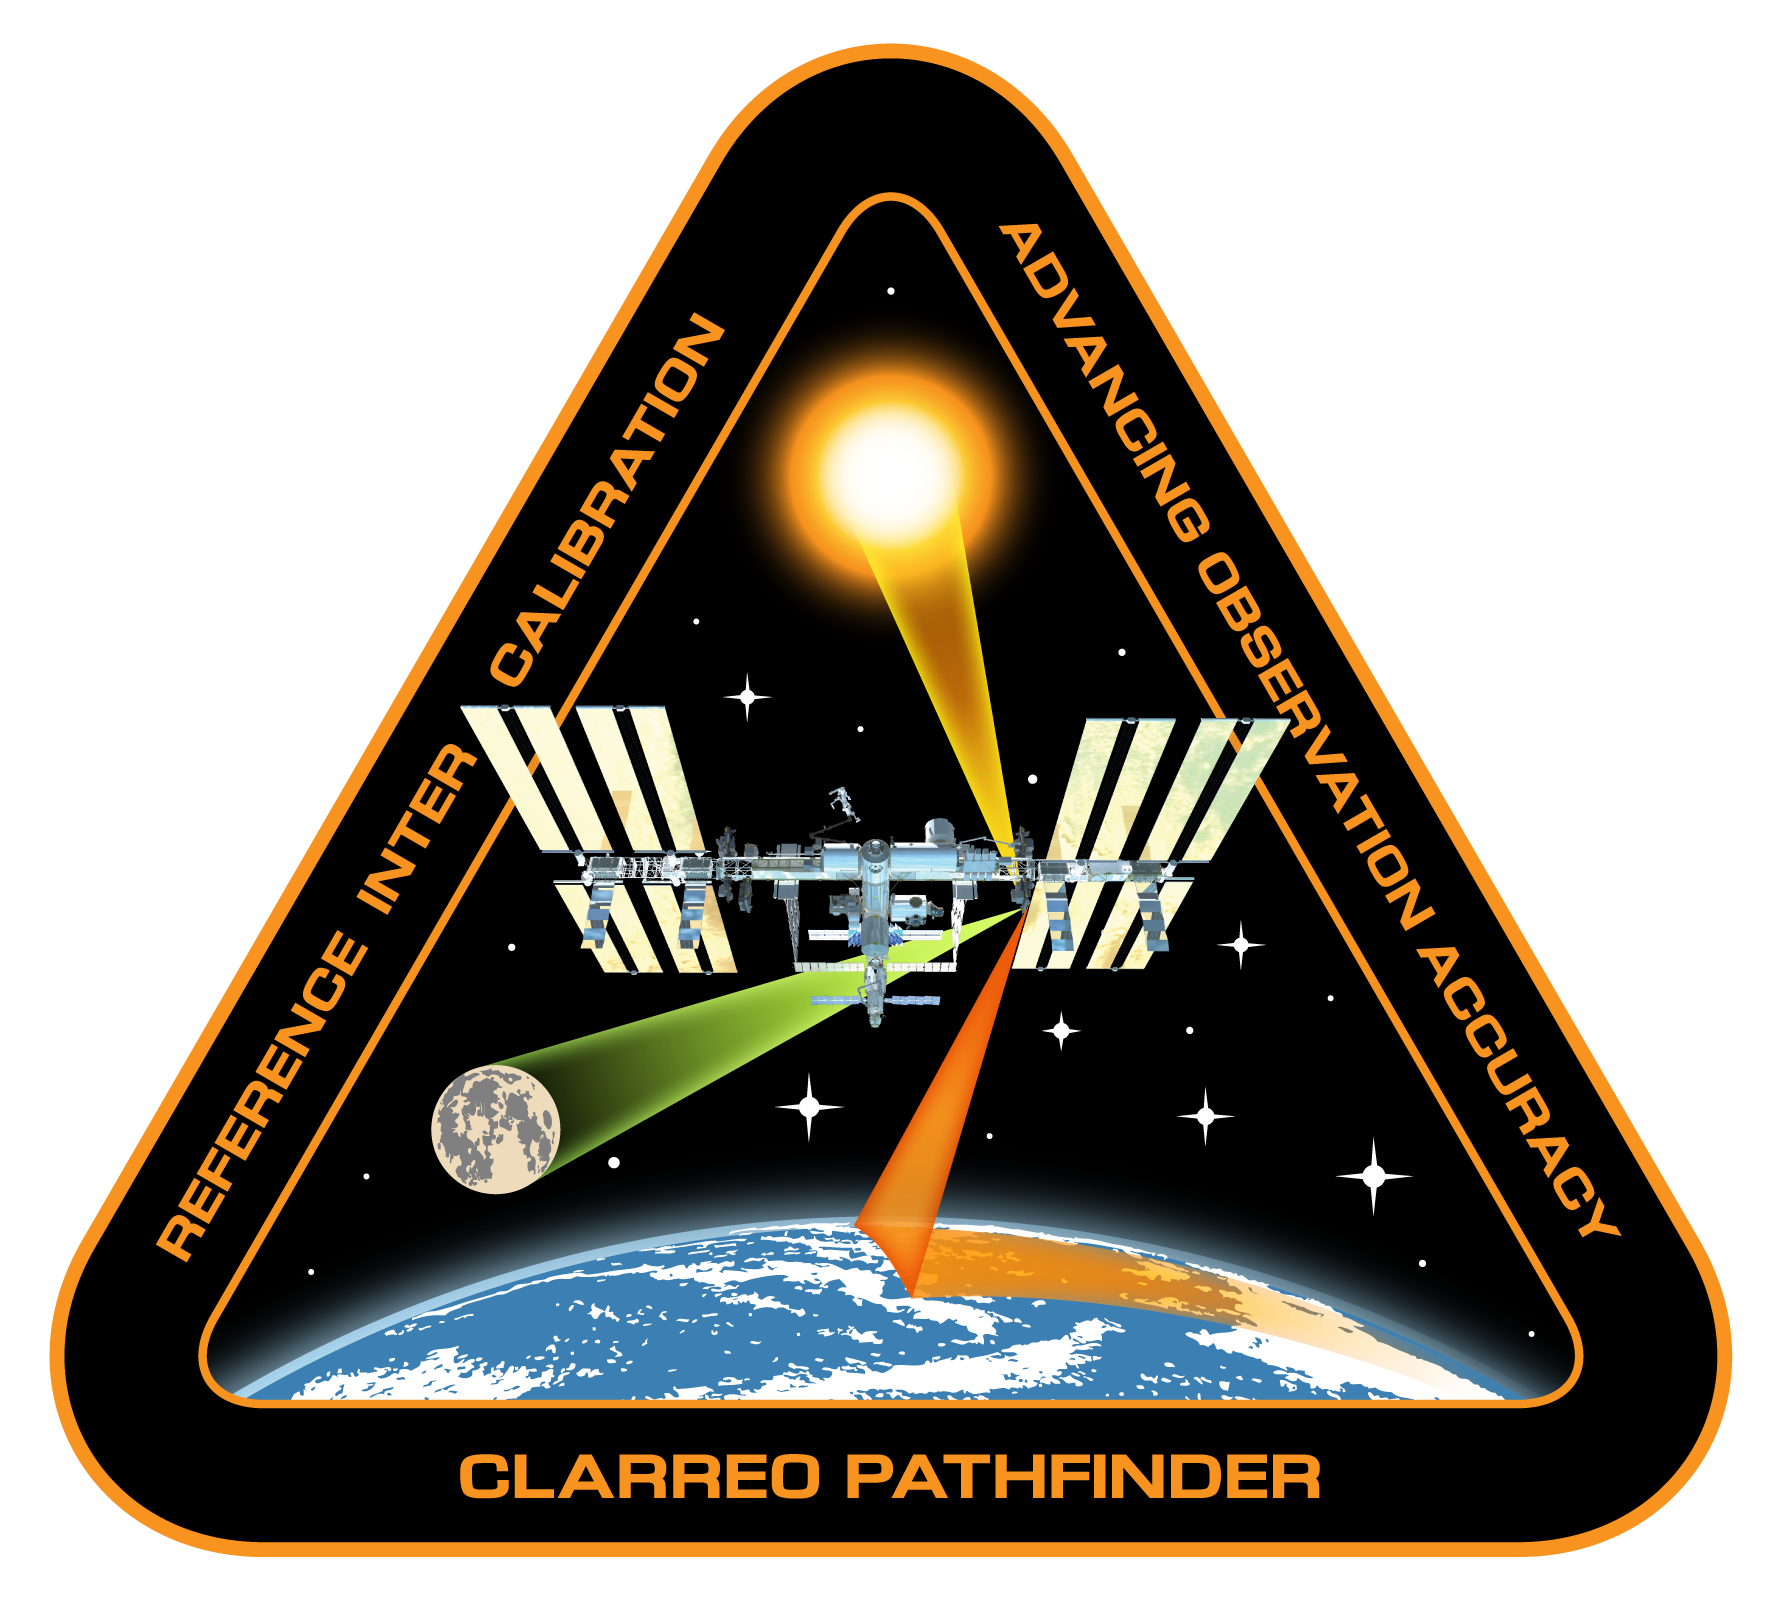
\includegraphics[keepaspectratio,width=2.3in]{cpf_logo.png}

\Large\bfseries
	Climate Absolute Radiance and Refractivity Observatory (CLARREO) Pathfinder \\
\vspace{0.4in}
\mytitle
\normalsize
\vspace{0.25in}
\mydate \\
\normalfont
\vspace{0.05in}
\fbox{
\begin{minipage}[t][9\height][c]{\dimexpr\textwidth-2\fboxsep-2\fboxrule\relax}
\centering
Approved for Public Release; Distribution is Unlimited
\end{minipage}
}
\clearpage

% Signature Page
% \bfseries
% \sffamily
% \center{\large SIGNATURE PAGE\par}
% \vspace{0.1in}
% \raggedright
% \normalfont
% \begin{table}[htbp]
% \begin{minipage}{\linewidth}
% \centering
% \small
% \begin{tabulary}{\textwidth}{p{3.325in}p{0.225in}p{2.5in}}
% \bfseries{~Prepared By:} & & \\[0.35in]
% \cmidrule(l){1-1}\cmidrule(l){3-3}
% ~Craig Hutchinson & & Tim Holden (LASP)\\
% ~Mission Architect & & Instrument Systems Engineer\\[0.25in]
% % \cmidrule(l){1-1}\cmidrule(l){3-3}
% % Name & & Name \\
% % Title & & Title \\[0.4in]
% \bfseries{~Concurred By:} & & \\[0.35in]
% \cmidrule(l){1-1}%\cmidrule(l){3-3}
% ~Jim Corliss & &  \\
% ~Science Manager & &  \\[0.35in]
% \cmidrule(l){1-1}%\cmidrule(l){3-3}
% ~Brian Boland & &  \\
% ~Systems Engineer & &  \\[0.35in]
% \cmidrule(l){1-1}%\cmidrule(l){3-3}
% ~Garfield Creary & &  \\
% ~Chief Engineer & &  \\[0.25in]
% \bfseries{~Approved By:} & & \\[0.35in]
% \cmidrule(l){1-1}%\cmidrule(l){3-3}
% ~Gary Fleming & &  \\
% ~Project Manager & &  \\[0.4in]
% % \cmidrule(l){1-1}\cmidrule(l){3-3}Name & & Name \\
% % Title & & Title \\[0.4in]
% \end{tabulary}
% \end{minipage}
% \end{table}
% \clearpage
% % Signature page for CLARREO Pathfinder SMRD
\bfseries
\sffamily
\center{\large SIGNATURE PAGE\par}
\vspace{0.1in}
\raggedright
\normalfont
\begin{table}[htbp]
\begin{minipage}{\linewidth}
\centering
\small
\begin{tabulary}{\textwidth}{p{3.325in}p{0.225in}p{2.5in}}
\bfseries{~Prepared By:} & & \\[0.35in]
~Electronic Approval on File\qquad\qquad\qquad2/21/2018\\
\cmidrule(l){1-1}%\cmidrule(l){3-3}
~Craig Hutchinson\\
~Systems Engineer\\[0.25in]
% \cmidrule(l){1-1}\cmidrule(l){3-3}
% Name & & Name \\
% Title & & Title \\[0.4in]
\bfseries{~Concurred By:} & & \\[0.35in]
~Electronic Approval on File\qquad\qquad\qquad3/1/2018\\
\cmidrule(l){1-1}%\cmidrule(l){3-3}
~Brian Boland & &  \\
~Lead Systems Engineer & &  \\[0.35in]
\bfseries{~Approved By:} & & \\[0.35in]
~Electronic Approval on File\qquad\qquad\qquad3/14/2018\\
\cmidrule(l){1-1}%\cmidrule(l){3-3}
~James Corliss & &  \\
~Chief Engineer & &  \\[0.35in]
~Electronic Approval on File\qquad\qquad\qquad2/27/2018\\
\cmidrule(l){1-1}%\cmidrule(l){3-3}
~Gary Fleming & &  \\
~Project Manager & &  \\[0.35in]
~Electronic Approval on File\qquad\qquad\qquad3/9/2018\\
\cmidrule(l){1-1}%\cmidrule(l){3-3}
~Bruce Wieliecki & &  \\
~Project Scientist & &  \\[0.4in]
% \cmidrule(l){1-1}\cmidrule(l){3-3}Name & & Name \\
% Title & & Title \\[0.4in]
\end{tabulary}
\end{minipage}
\end{table}
\clearpage
% ***Begin: sig_page
% Signature page for CLARREO Pathfinder SMRD
\bfseries
\sffamily
\center{\large SIGNATURE PAGE\par}
\vspace{0.1in}
\raggedright
\normalfont
\begin{table}[htbp]
\begin{minipage}{\linewidth}
\centering
\small
\begin{tabulary}{\textwidth}{p{3.325in}p{0.225in}p{2.5in}}
\bfseries{~Prepared By:} & & \\[0.35in]
 \\
\cmidrule(l){1-1}%\cmidrule(l){3-3}
~Craig Hutchinson\\
~Systems Engineer\\[0.25in]
% \cmidrule(l){1-1}\cmidrule(l){3-3}
% Name & & Name \\
% Title & & Title \\[0.4in]
\bfseries{~Concurred By:} & & \\[0.35in]
 \\
\cmidrule(l){1-1}\cmidrule(l){3-3}
~Stephen Bowen & & ~Brian Boland \\
~Power Converter Unit Subsystem Lead & & ~Lead Systems Engineer \\[0.35in]
 \\
\cmidrule(l){1-1}\cmidrule(l){3-3}
~Aref Nammari & & ~Ryan Lewis \\
~CPRS Electrical Lead at LASP & & ~CPRS Mechanical Lead at LASP \\[0.35in]
\bfseries{~Approved By:} & & \\[0.35in]
 \\
\cmidrule(l){1-1}%\cmidrule(l){3-3}
~James Corliss & &  \\
~Chief Engineer & &  \\[0.35in]
 \\
\cmidrule(l){1-1}%\cmidrule(l){3-3}
~Gary Fleming & &  \\
~Project Manager & &  \\[0.35in]
\end{tabulary}
\end{minipage}
\end{table}
\clearpage% ***End: sig_page

% Revision History and TBX Table Page
% \sffamily
% \bfseries
% \center{\large REVISION HISTORY PAGE\par}
% \normalfont
% \centering
% \begin{table}[htbp]
% \begin{minipage}{\linewidth}
% \setlength{\tymax}{0.5\linewidth}
% \centering
% \small
% \begin{tabular}{| >{\centering\arraybackslash}m{1.25in}| >{\centering\arraybackslash}m{2.95in}| >{\centering\arraybackslash}m{1.5in}|} \hline
% \bfseries{Revision No.} & \bfseries{Description} & \bfseries{Release Date}\\
% \hline
% Preliminary & Mission Concept Review & N/A \\
% \hline
% \revision & System Requirements and Mission Definition Review & \releasedate \\
% \hline
% \end{tabular}
% % \end{tabulary}
% \end{minipage}
% \end{table}
% 
            \clearpage
            \sffamily
            \bfseries
            \center{\large TBX LIST\par}
            \normalfont
            \centering
            \begin{table}[htbp]
            \begin{minipage}{\linewidth}
            \setlength{\tymax}{0.5\linewidth}
            \centering
            \small\begin{tabular}{| >{\centering\arraybackslash}m{1.25in}| >{\centering\arraybackslash}m{2.95in}| >{\centering\arraybackslash}m{1.5in}|} \hline
            \bfseries{Item} & \bfseries{Description} & \bfseries{Page}\\
            \hline
            TBR & Delivery destination and role of PCU in CPRSP testing & \pageref{tbx_1}  \\ 
 \hline 
TBR & Pending thermal analysis of whether survival heaters are necessary for PCU & \pageref{tbx_2}  \\ 
 \hline 
TBR & Pending thermal analysis of whether there is thermal interface with Adaptor Plate & \pageref{tbx_3}  \\ 
 \hline 
TBR & Voltage of Discrete Input Signals & \pageref{tbx_4}  \\ 
 \hline 
TBR & Value of Bus A maximum current & \pageref{tbx_5}  \\ 
 \hline 
TBR & Value of Bus B maximum current & \pageref{tbx_6}  \\ 
 \hline 
TBR & Value of Bus C maximum current & \pageref{tbx_7}  \\ 
 \hline 
TBD & Drawing from LASP showing PCU positioning on ExPA & \pageref{tbx_8}  \\ 
 \hline 
TBD & Molecular Deposition onto Other Payloads Limit & \pageref{tbx_9}  \\ 
 \hline 
TBD & Molecular Deposition onto Other ISS Elements Limit & \pageref{tbx_10}  \\ 
 \hline 
TBD & Axial Launch Load Limit & \pageref{tbx_11}  \\ 
 \hline 
TBD & Lateral Launch Load Limit & \pageref{tbx_12}  \\ 
 \hline 
TBR & Minimum Natural Frequency & \pageref{tbx_13}  \\ 
 \hline 
TBD & Tolerance of thermal mass & \pageref{tbx_14}  \\ 
 \hline 
TBD & Thermal Testing Temperature & \pageref{tbx_15}  \\ 
 \hline 
\end{tabular}
        \end{minipage}
        \end{table}
        \raggedright
        \clearpage
% \clearpage
% % CLARREO Pathfinder SMRD Revision History and TBX Table Page for non-Supplemental document
\sffamily
\bfseries
\center{\large REVISION HISTORY PAGE\par}
\normalfont
\centering
\begin{table}[htbp]
\begin{minipage}{\linewidth}
\setlength{\tymax}{0.5\linewidth}
\centering
\small
\begin{tabular}{| >{\centering\arraybackslash}m{1.25in}| >{\centering\arraybackslash}m{2.95in}| >{\centering\arraybackslash}m{1.5in}|} \hline
\bfseries{Revision No.} & \bfseries{Description} & \bfseries{Release Date}\\
\hline
Baseline & Baseline. See CPF-CR-007 & 29 June 2017 \\
\hline
A & See CPF-CR-011 & 17 January 2018 \\
\hline
B & See CPF-CR-012 & 14 March 2018 \\
\hline
C & See CPF-CR-013 & \releasedate \\
\hline
\end{tabular}
% \end{tabulary}
\end{minipage}
\end{table}

            \clearpage
            \sffamily
            \bfseries
            \center{\large TBX LIST\par}
            \normalfont
            \centering
            \begin{table}[htbp]
            \begin{minipage}{\linewidth}
            \setlength{\tymax}{0.5\linewidth}
            \centering
            \small\begin{tabular}{| >{\centering\arraybackslash}m{1.25in}| >{\centering\arraybackslash}m{2.95in}| >{\centering\arraybackslash}m{1.5in}|} \hline
            \bfseries{Item} & \bfseries{Description} & \bfseries{Page}\\
            \hline
            TBR & Delivery destination and role of PCU in CPRSP testing & \pageref{tbx_1}  \\ 
 \hline 
TBR & Pending thermal analysis of whether survival heaters are necessary for PCU & \pageref{tbx_2}  \\ 
 \hline 
TBR & Pending thermal analysis of whether there is thermal interface with Adaptor Plate & \pageref{tbx_3}  \\ 
 \hline 
TBR & Voltage of Discrete Input Signals & \pageref{tbx_4}  \\ 
 \hline 
TBR & Value of Bus A maximum current & \pageref{tbx_5}  \\ 
 \hline 
TBR & Value of Bus B maximum current & \pageref{tbx_6}  \\ 
 \hline 
TBR & Value of Bus C maximum current & \pageref{tbx_7}  \\ 
 \hline 
TBD & Drawing from LASP showing PCU positioning on ExPA & \pageref{tbx_8}  \\ 
 \hline 
TBD & Molecular Deposition onto Other Payloads Limit & \pageref{tbx_9}  \\ 
 \hline 
TBD & Molecular Deposition onto Other ISS Elements Limit & \pageref{tbx_10}  \\ 
 \hline 
TBD & Axial Launch Load Limit & \pageref{tbx_11}  \\ 
 \hline 
TBD & Lateral Launch Load Limit & \pageref{tbx_12}  \\ 
 \hline 
TBR & Minimum Natural Frequency & \pageref{tbx_13}  \\ 
 \hline 
TBD & Tolerance of thermal mass & \pageref{tbx_14}  \\ 
 \hline 
TBD & Thermal Testing Temperature & \pageref{tbx_15}  \\ 
 \hline 
\end{tabular}
        \end{minipage}
        \end{table}
        \raggedright
        \clearpage
\clearpage

% ***Begin: rev_hist_compile
% CLARREO Pathfinder SMRD Revision History and TBX Table Page for non-Supplemental document
\sffamily
\bfseries
\center{\large REVISION HISTORY PAGE\par}
\normalfont
\centering
\begin{table}[htbp]
\begin{minipage}{\linewidth}
\setlength{\tymax}{0.5\linewidth}
\centering
\small
\begin{tabular}{| >{\centering\arraybackslash}m{1.25in}| >{\centering\arraybackslash}m{2.95in}| >{\centering\arraybackslash}m{1.5in}|} \hline
\bfseries{Revision No.} & \bfseries{Description} & \bfseries{Release Date}\\
\hline
Preliminary & Draft Work in Progress & TBD \\
\hline
\end{tabular}
% \end{tabulary}
\end{minipage}
\end{table}
% 
            \clearpage
            \sffamily
            \bfseries
            \center{\large TBX LIST\par}
            \normalfont
            \centering
            \begin{table}[htbp]
            \begin{minipage}{\linewidth}
            \setlength{\tymax}{0.5\linewidth}
            \centering
            \small\begin{tabular}{| >{\centering\arraybackslash}m{1.25in}| >{\centering\arraybackslash}m{2.95in}| >{\centering\arraybackslash}m{1.5in}|} \hline
            \bfseries{Item} & \bfseries{Description} & \bfseries{Page}\\
            \hline
            TBR & Delivery destination and role of PCU in CPRSP testing & \pageref{tbx_1}  \\ 
 \hline 
TBR & Pending thermal analysis of whether survival heaters are necessary for PCU & \pageref{tbx_2}  \\ 
 \hline 
TBR & Pending thermal analysis of whether there is thermal interface with Adaptor Plate & \pageref{tbx_3}  \\ 
 \hline 
TBR & Voltage of Discrete Input Signals & \pageref{tbx_4}  \\ 
 \hline 
TBR & Value of Bus A maximum current & \pageref{tbx_5}  \\ 
 \hline 
TBR & Value of Bus B maximum current & \pageref{tbx_6}  \\ 
 \hline 
TBR & Value of Bus C maximum current & \pageref{tbx_7}  \\ 
 \hline 
TBD & Drawing from LASP showing PCU positioning on ExPA & \pageref{tbx_8}  \\ 
 \hline 
TBD & Molecular Deposition onto Other Payloads Limit & \pageref{tbx_9}  \\ 
 \hline 
TBD & Molecular Deposition onto Other ISS Elements Limit & \pageref{tbx_10}  \\ 
 \hline 
TBD & Axial Launch Load Limit & \pageref{tbx_11}  \\ 
 \hline 
TBD & Lateral Launch Load Limit & \pageref{tbx_12}  \\ 
 \hline 
TBR & Minimum Natural Frequency & \pageref{tbx_13}  \\ 
 \hline 
TBD & Tolerance of thermal mass & \pageref{tbx_14}  \\ 
 \hline 
TBD & Thermal Testing Temperature & \pageref{tbx_15}  \\ 
 \hline 
\end{tabular}
        \end{minipage}
        \end{table}
        \raggedright
        \clearpage
% ***Begin: tbx_table

            \clearpage
            \sffamily
            \bfseries
            \center{\large TBX LIST\par}
            \normalfont
            \centering
            \begin{table}[htbp]
            \begin{minipage}{\linewidth}
            \setlength{\tymax}{0.5\linewidth}
            \centering
            \small\begin{tabular}{| >{\centering\arraybackslash}m{1.25in}| >{\centering\arraybackslash}m{2.95in}| >{\centering\arraybackslash}m{1.5in}|} \hline
            \bfseries{Item} & \bfseries{Description} & \bfseries{Page}\\
            \hline
            TBR & Delivery destination and role of PCU in CPRSP testing & \pageref{tbx_1}  \\ 
 \hline 
TBR & Pending thermal analysis of whether survival heaters are necessary for PCU & \pageref{tbx_2}  \\ 
 \hline 
TBR & Pending thermal analysis of whether there is thermal interface with Adaptor Plate & \pageref{tbx_3}  \\ 
 \hline 
TBR & Voltage of Discrete Input Signals & \pageref{tbx_4}  \\ 
 \hline 
TBR & Value of Bus A maximum current & \pageref{tbx_5}  \\ 
 \hline 
TBR & Value of Bus B maximum current & \pageref{tbx_6}  \\ 
 \hline 
TBR & Value of Bus C maximum current & \pageref{tbx_7}  \\ 
 \hline 
TBD & Drawing from LASP showing PCU positioning on ExPA & \pageref{tbx_8}  \\ 
 \hline 
TBD & Molecular Deposition onto Other Payloads Limit & \pageref{tbx_9}  \\ 
 \hline 
TBD & Molecular Deposition onto Other ISS Elements Limit & \pageref{tbx_10}  \\ 
 \hline 
TBD & Axial Launch Load Limit & \pageref{tbx_11}  \\ 
 \hline 
TBD & Lateral Launch Load Limit & \pageref{tbx_12}  \\ 
 \hline 
TBR & Minimum Natural Frequency & \pageref{tbx_13}  \\ 
 \hline 
TBD & Tolerance of thermal mass & \pageref{tbx_14}  \\ 
 \hline 
TBD & Thermal Testing Temperature & \pageref{tbx_15}  \\ 
 \hline 
\end{tabular}
        \end{minipage}
        \end{table}
        \raggedright
        \clearpage% ***End: tbx_table
\clearpage
% ***End: rev_hist_compile

\glsunsetall
\normalfont
\setlength{\beforechapskip}{-16pt}
\setcounter{tocdepth}{5}
\tableofcontents*
\setlength{\beforechapskip}{6pt}
\apptoc
\listoftables*
\listoffigures*
\glsresetall
\clearpage

\setcounter{secnumdepth}{5}
\setlist[enumerate,1]{label=\arabic*., ref=\arabic*}

\raggedright
\setlength{\parskip}{\baselineskip}
\chapterstyle{cpf}% ***End: mmd6-cpf-front-matter
% % List of acronyms that tend to be nested. This enables LaTeX to reliably expand acronyms
\newacronym{OTCM}{OTCM}{\gls{ORU} Tool Changeout Mechanism}
\newacronym{EOTP}{EOTP}{Enhanced \gls{ORU} Temporary Platform}
% ***Begin: nestedacros
% List of acronyms that tend to be nested. This enables LaTeX to reliably expand acronyms
\newacronym{OTCM}{OTCM}{\gls{ORU} Tool Changeout Mechanism}
\newacronym{EOTP}{EOTP}{Enhanced \gls{ORU} Temporary Platform}% ***End: nestedacros




% ***End: mmd6-cpf-begin

\chapter{Introduction }
\label{introduction}

\section{Purpose and Scope }
\label{purposeandscope}

This document establishes the \gls{PCU} requirements, which specify the subsystem that converts 120 \gls{VDC} Operational Power to 28 \gls{VDC} power suitable for the other \gls{CPRSP} subsystems.

\section{Document Organization }
\label{documentorganization}

\autoref{sec_docs} lists applicable and reference documents. \autoref{conops} provides the \gls{PCU} concept of operations. \autoref{interfaces} discusses the external interfaces and boundaries of the \gls{PCU}. \autoref{sec_req} contains the technical requirements. Appendix A defines acronyms.

\chapter{Documents  }
\label{sec_docs}

This section identifies documents that are applicable to this document and assumes the current version unless otherwise noted. Reference documents are for information only.

\section{Applicable Documents }
\label{applicabledocuments}


% Double vertical bar above is kludge to get around python code bug


\begin{table}[htbp]
\begin{minipage}{\linewidth}
\setlength{\tymax}{0.5\linewidth}
\centering
\small
\begin{tabulary}{\textwidth}{|+p{1.8in}|^p{4.2in}|} \hline
\rowstyle{\bfseries}%
 Document Number & Document Title \\
\hline

 \gls{CPF}--02--002 & \gls{CLARREO} Pathfinder Systems Engineering Management Plan \\
 \gls{CPF}--02--009 & \gls{CLARREO} Pathfinder Mission Concept of Operations \\
 \gls{CPF}--02--011 & \gls{CLARREO} Pathfinder Science and Mission Requirements Document \\
 \gls{CPF}--03--001 & \gls{CLARREO} Pathfinder Mission Assurance Requirements \\
 \gls{LASP} Document No. 154920 & \gls{CLARREO}--Pathfinder \gls{PCU} Electrical Interface Control Document \\
\hline

\end{tabulary}
\end{minipage}
\end{table}

\section{Reference Documents }
\label{referencedocuments}


% Double vertical bar above is kludge to get around python code bug


\begin{table}[htbp]
\begin{minipage}{\linewidth}
\setlength{\tymax}{0.5\linewidth}
\centering
\small
\begin{tabulary}{\textwidth}{|+p{1.8in}|^p{4.2in}|} \hline
\rowstyle{\bfseries}%
 Document Number & Document Title \\
\hline

 D683--9747--01 Revision E & Expedite the Processing of Experiments to Space Station (ExPRESS) Pallet Adapter (ExPA) Interface Definition Document (IDD) \\
 \gls{GSFC}--STD--7000A & General Environmental Verification Standard \\
 SpX--00036031 & Dragon \gls{FRAM} Payloads Interface Requirements Document (IRD) \\
 SSP 30237 & Space Station Electromagnetic Emission and Susceptibility Requirements \\
 SSP 30245 & Space Station Electrical Bonding Requirements \\
 SSP 30512 & Space Station Ionizing Radiation Design Environment \\
 SSP 51700 & Payload Safety Policy and Requirements for the International Space Station \\
 SSP 52005 & Payload Flight Equipment Requirements and Guidelines for Safety--Critical Structures \\
 SSP 57003 Revision L & External Payload Interface Requirements Document \\
\hline

\end{tabulary}
\end{minipage}
\end{table}

\section{Document Control }
\label{documentcontrol}

This document is managed by the \gls{CPF} Project and, after initial approval, will be placed under configuration control using the change management processes defined in the \gls{CLARREO} Pathfinder Configuration Management Operating Procedure (CPF-01--005).

\section{Order of Precedence }
\label{orderofprecedence}

The Program-Level Requirements and Project-Level plans listed in the applicable documents section take precedence over the \gls{PCU} \gls{ICD}. Nothing in this document, however, supersedes applicable laws and regulations.

\chapter{Concept of Operations  }
\label{conops}

The Power Converter Unit is a part of the \gls{CPRSP}, along with the \gls{HISIE}, \gls{HPS}, \gls{HySICS} Instrument, and \gls{ExPA}. The \gls{PCU}'s primary role is to convert 120 \gls{VDC} Operational Power provided by the \gls{ELC} to 28 \gls{VDC} Power to service the remaining elements of the \gls{CPRSP} when the discrete data input is activated.

The \gls{PCU} operates in a host of different scenarios during its lifetime from integration through disposal. Following assembly, the \gls{PCU} completes functional and environmental testing at \gls{LaRC}.

The \gls{PCU} is shipped to \gls{LASP}, where it is functionally tested with the \gls{CPRSP} subsystems other than the the \gls{ExPA} (TBR\label{tbx_1}). The 28 \gls{VDC} output of the \gls{PCU} is connected to the \gls{HISIE} and \gls{HPS} via three buses and connect 120 \gls{VDC} and discrete data test lines to the \gls{PCU}'s input ports. The \gls{PCU} provides analog signal and thermistor outputs to enable troubleshooting and monitoring of \gls{PCU} operations during \gls{CPRSP} testing at \gls{LASP}, all other ground testing, and on-orbit operations. The \gls{PCU} may be used during thermal vacuum chamber testing. As a programmatic alternative to integration with the other \gls{CPRSP} elements at \gls{LASP}, the \gls{PCU} may travel directly from \gls{LaRC} to Kennedy Space Center for subsequent \gls{CPRSP} integration.

After completion of the testing at \gls{KSC}, the \gls{PCU} remains unpowered until the \gls{CPRSP} is attached to \gls{ELC}-1. During installation when the \gls{CPRSP} is attached to the \gls{EOTP}, the discrete is not asserted, and the \gls{PCU} does not draw power from the \gls{EOTP}.

Following installation, the \gls{PCU} power is nominally enabled by \gls{ISS} controllers performing two actions. The first action is activating the 120 \gls{VDC} Operational Power bus, allowing that power to flow via the J1 port on the \gls{ExPA}. The relay's switch is normally open and closes only when the discrete data line is activated. The second action is activating the commanding discrete, at which point the \gls{PCU} energizes the voltage conversion circuitry to output 28 \gls{VDC}.

When either the 120 \gls{VDC} Operational Power is removed or the discrete data line is deactivated, the \gls{PCU} ceases outputting 28 \gls{VDC} power. When science operations are complete or for other scenarios requiring planned deactivation of the \gls{PCU}, the nominal order of controller operations for de-energizing the \gls{PCU} is deactivating the commanding discrete, followed by deactivating the 120 \gls{VDC} Operational Power bus. In the event of an unplanned power outage of the 120 \gls{VDC} Operational Bus, controllers deactivate the commanding discrete as soon as possible if power had not yet been restored. Both planned and unplanned power outages remove all power to the \gls{CPRSP}.

\chapter{External Interfaces  }
\label{interfaces}

\section{External Interfaces by Function}
\label{externalinterfacesbyfunction}

The \gls{PCU} maintains external interfaces across the following functions:

\begin{itemize}
\item{} Structural

\begin{itemize}
\item{} \gls{ExPA} Attachment

\end{itemize}

\item{} Power

\begin{itemize}
\item{} 28V Power Output

\begin{itemize}
\item{} 28 \gls{VDC} Bus A Power Out

\item{} 28 \gls{VDC} Bus B Power Out

\item{} 28 \gls{VDC} Bus C Power Out

\end{itemize}

\item{} 120V Power Input

\end{itemize}

\item{} Data or signal

\begin{itemize}
\item{} Analog Signals \slash  Thermistor Output

\begin{itemize}
\item{} Thermistor Out x 6

\item{} Bus A Current Analog Out

\item{} Bus B Current Analog Out

\item{} Bus C Current Analog Out

\item{} Bus Voltage Analog Out

\end{itemize}

\end{itemize}

\item{} Thermal

\begin{itemize}
\item{} \gls{ExPA} Heat Rejection

\item{} Survival Heaters (TBR\label{tbx_2})

\item{} Adaptor Plate (TBR\label{tbx_3})

\end{itemize}

\item{} Command

\begin{itemize}
\item{} Discrete Enable Input

\end{itemize}

\end{itemize}

\section{External Interface Boundaries}
\label{externalinterfaceboundaries}

\autoref{boundaries} shows the boundaries between each of the external interfaces. The External Subsystem identifies the subsystem to which the \gls{PCU} shares an interface. \gls{CPRSP} ancillary refers to hardware that is not yet specifically allocated to \gls{CPRSP} subsystems, generally the wiring harnesses in the context of the \gls{PCU}. The \gls{PCU} Items belong to, and will be delivered with the \gls{PCU}. The External Items belong to the External Subsystem, and the \gls{PCU} design assumes their presence and availability for connection. \gls{LASP} Document Number 154920 provides specific pinout information on the interfaces with the \gls{CPRSP} ancillary external item.




\begin{table}[htbp]
\begin{minipage}{\linewidth}
\setlength{\tymax}{0.5\linewidth}
\centering
\small
\caption{External Interface Boundaries}
\label{boundaries}
\begin{tabulary}{\textwidth}{|+p{2.5in}|^p{1.5in}|^p{0.7in}|^p{1.25in}|} \hline
\rowstyle{\bfseries}%
 Interface & External Subsystem & \gls{PCU} Item & External Item \\
\hline

 \gls{ExPA} Attachment & \gls{ExPA} & Holes & Fasteners \\
 28V Power Output (J20) & \gls{CPRSP} ancillary & \gls{PCU} Jack & Mating Connector \\
 120V Power Input (J21) & \gls{CPRSP} ancillary & \gls{PCU} Jack & Mating Connector \\
 Analog Signals \slash  Thermistor Output (J22) & \gls{CPRSP} ancillary & \gls{PCU} Jack & Mating Connector \\
 Discrete Enable Input (J23) & \gls{CPRSP} ancillary & \gls{PCU} Jack & Mating Connector \\
 \gls{ExPA} Thermal & \gls{ExPA} & \gls{PCU} \texttt{-Z} surface & \gls{ExPA} surface \\
 Survival Heaters (TBR) & \gls{CPRSP} ancillary & \gls{PCU} surface & Survival Heater \\
 Adaptor Plate Thermal (TBR) & \gls{CPRSP} ancillary & \gls{PCU} \texttt{+Z} surface & Adaptor Plate \\
\hline

\end{tabulary}
\end{minipage}
\end{table}

\chapter{Requirements  }
\label{sec_req}

\renewcommand\labelitemi{}

This section contains the requirements that define the performance of the \gls{PCU}, its interface with the other \gls{CPRSP} subsystems, and the testing of the delivered article.

\section{Accepts 120 VDC Input}
\label{accepts120vdcinput}

\textbf{[PCU.10000]} Input 120 \gls{VDC}

The \gls{PCU} shall operate nominally given a steady-state voltage between 106.5 \gls{VDC} and 126.5 \gls{VDC} on the Operational Power input in accordance with \gls{LASP} Document No. 154920.

\begin{itemize}
\item{} Rationale: \emph{The PCU converts the 120 VDC Operational Power supplied by the ExPA into 28 VDC. Document No. 154920 identifies the pins, part number, manufacturer, and description of the 120V Power Input interface jack and mating connector. This derives from the ELC 120 VDC Power Interface requirements of section E.3.2.1.1.1 of SSP 57003 Rev L. Figure E.3.2.1.1.2--1 implies that the PCU could see a minimum of 102 VDC.}

\end{itemize}

\textbf{[PCU.10005]} Exposure to Brownout

The \gls{PCU} shall operate nominally after exposure to input voltages from 0 to 120 \gls{VDC} during brownout.

\begin{itemize}
\item{} Rationale: \emph{The PCU needs to be resilient to times when the ELC may provide less voltage than the advertised nominal value.}

\item{} Comments: \textbf{What is the LASP rationale for this requirement? Given the nominal input voltage range of 102V-126.5V, the brownout range cannot be all the way up to 120V. It seems like there should be more specifics to account for a particular condition. How does LASP want LaRC to verify this requirement?}

\end{itemize}

\textbf{[PCU.10010]} Survival Following Unannounced Removal of Power

The \gls{PCU} shall survive after exposure to an unplanned removal of power.

\begin{itemize}
\item{} Rationale: \emph{The PCU needs to be resilient to times when the ISS removes 120V Operational Power from the ELC prior to notifying the CPOC due to operational constraints.}

\end{itemize}

\textbf{[PCU.10015]} Protection from Input Polarity Reversal

The \gls{PCU} shall protect itself from damage due to reversed polarity at the \gls{PCU} 120 \gls{VDC} input.

\begin{itemize}
\item{} Rationale: \emph{During integration and test, there is a possibility that technicians may attach the wrong connectors to the 120 VDC inputs, and the PCU design need to accommodate this situation.}

\end{itemize}

\textbf{[PCU.10020]} 120 \gls{VDC} Non-Normal Voltage Transients

The \gls{PCU} shall operate nominally following exposure to transient voltage conditions as specified by SSP 57003 Rev L Figure E.3.2.1.1.2--1.

\begin{itemize}
\item{} Rationale: \emph{This requirement protects the ISS in the event of a transient voltage condition. Loads may be exposed to transient overvoltage conditions during operation of the power system's fault protection components. This derives from the ELC 120 VDC Power Interface requirements of section E.3.2.1.1.2 of SSP 57003 Rev L.}

\end{itemize}

\textbf{[PCU.10025]} Reverse Current

The \gls{PCU} shall limit reverse current transients in accordance with Figures E.3.2.1.1.4--1, E.3.2.1.1.4--2, E.3.2.1.1.4--3 of SSP 57003 Rev L when exposed to a hard fault across the power source, as specified by section E.3.2.1.1.4 of SSP 57003 Rev L.

\begin{itemize}
\item{} Rationale: \emph{This requirement prevents current from entering an output and damaging components. For purposes of this interface definition, the fault is 10 milliohms or less applied within 2 micro-seconds or less. For the ELC Payload\slash payload exhibiting reverse current transient peaks within +\slash -100 Amperes, the fault resistance is 40 milliohms or less. This derives from the ELC 120 VDC Power Interface requirements of section E.3.2.1.1.4 of SSP 57003 Rev L.}

\end{itemize}

\textbf{[PCU.10030]} 120 \gls{VDC} Operational Power Ripple Voltage and Noise

The \gls{PCU} shall operate and be compatible with the EPS time domain ripple voltage and noise level of 2.5 Vrms maximum within the frequency range of 30 Hz to 1 MH when connected to 120 \gls{VDC} Operational Power.

\begin{itemize}
\item{} Rationale: \emph{This requirement precludes damage to ExPCA and ORUs. Derives from the ELC 120 VDC Power Interface requirements of section E.3.2.1.1.6.2 of SSP 57003 Rev L.}

\end{itemize}

\textbf{[PCU.10035]} 120 \gls{VDC} Operational Power Ripple Voltage Spectrum

The \gls{PCU}, connected to \gls{ELC} 120 \gls{VDC} output, shall operate and be compatible with the EPS ripple voltage spectrum of a maximum as shown in SSP 57003 Rev L Figure E.3.2.1.1.6.3--1.

\begin{itemize}
\item{} Rationale: \emph{This requirement precludes damage to ExPCA and ORUs. Note: This limit is 6 decibels (dB) below the Electromagnetic Compatibility (EMC) CS-01, 02 requirement in SSP 30237, Space Station Requirements for Electromagnetic Emission and Susceptibility Requirements, up to 30 MHz. Derives from the ELC 120 VDC Power Interface requirements of section E.3.2.1.1.6.3 of SSP 57003 Rev L.}

\end{itemize}

\textbf{[PCU.10040]} 120 \gls{VDC} Operational Power Surge Current

The \gls{PCU} shall limit in-rush current at power input connected to \gls{ELC} 120 \gls{VDC} output interface in accordance with Table E.3.2.1.1.6.4--1 of SSP 57003 Rev L.

\begin{itemize}
\item{} Rationale: \emph{This requirement prevents a hazard due to circuit overload. Derives from the ELC 120 VDC Power Interface requirements of section E.3.2.1.1.6.4 of SSP 57003 Rev L.}

\end{itemize}

\section{Accepts Discretes}
\label{acceptsdiscretes}

\textbf{[PCU.11000]} Input Discrete Power-on Command

The \gls{PCU} shall recognize a digital logic zero (VIL) and digital logic one (VIH) for +5 V or +28 V TBR\label{tbx_4} logic levels from the ExPCA as defined in Table L.3.7.4.1.1--1, Discrete Output Logic Levels, between the payload input pins.

\begin{itemize}
\item{} Rationale: \emph{The discrete signal conveys the power on command to the PCU. Document No. 154920 identifies the pins, part number, manufacturer, and description of the Discrete Enable Input interface jack and mating connector. Derives from Discrete Output Logic Levels (from ExPCA) requirements of section L.3.7.4.1.1 of SSP 57003 Rev L.}

\end{itemize}

\textbf{[PCU.11005]} Output Power with Discrete Present

The \gls{PCU} shall activate its output voltage when the discrete Power-on signal is logic one and when 120 \gls{VDC} is applied to the \gls{PCU} input.

\begin{itemize}
\item{} Rationale: \emph{The PCU output power is normally off and enabled when the discrete signal is present (logic one).}

\end{itemize}

\textbf{[PCU.11010]} No Output Power without Discrete

The \gls{PCU} shall cease outputting power when the discrete Power-on signal is logic zero.

\begin{itemize}
\item{} Rationale: \emph{The PCU output power is normally off and only enabled when the discrete signal is present (logic one). This prevents the PCU from drawing a significant load unless the CPRSP is attached to the ELC and commanded on by the CPOC.}

\end{itemize}

\textbf{[PCU.11015]} Discrete Returns

The \gls{PCU} shall provide an individual return for each \gls{ISS} low level discrete signal.

\begin{itemize}
\item{} Rationale: \emph{A dedicated return ensures that return currents are routed with supply leads, thus minimizing radiation due to differential mode currents and aids in crosstalk reduction. Not sharing returns minimizes the chances of common impedance noise coupling. This derives from the Analog, Differential Circuit Return requirement in section 3.2.3.3.2.6 of SSP 57003 Rev L.}

\end{itemize}

\textbf{[PCU.11020]} Discrete Loading - Capacitance

The \gls{PCU} shall prevent the maximum capacitive loading on the \gls{ExPA} discrete outputs from exceeding 1 microFarad.

\begin{itemize}
\item{} Rationale: \emph{This requirement ensures that discrete signals (including those used to control a hazard) are received. This derives from the Payload Discrete Loading Requirements in section L.3.7.4.6.A of SSP 57003 Rev L.}

\end{itemize}

\textbf{[PCU.11025]} Discrete Loading - Inductance

The \gls{PCU} shall prevent the maximum inductive loading the \gls{ExPA} discrete outputs from exceeding 10mH.

\begin{itemize}
\item{} Rationale: \emph{This requirement ensures that discrete signals (including those used to control a hazard) are received. This derives from the Payload Discrete Loading Requirements in section L.3.7.4.6.A of SSP 57003 Rev L.}

\end{itemize}

\textbf{[PCU.11031]} Discrete Loading - Resistance 28 V

The \gls{PCU} shall ensure that the maximum resistive loading on the ExPCA +28V discrete output exceeds 700 Ohm, except for when used for switch closure detection.

\begin{itemize}
\item{} Rationale: \emph{This requirement ensures that discrete signals (including those used to control a hazard) are received. The ExPCA discrete output voltage span of +28 Vdc +2.6\slash -4.0 Vdc is not guaranteed when loading exceeds 35mA (current-limiting will occur with FRAM-based Payload loads drawing about 35 mA). This derives from the Payload Discrete Loading Requirements in section L.3.7.4.6.B of SSP 57003 Rev L.}

\end{itemize}

\section{Outputs 28 VDC}
\label{outputs28vdc}

\textbf{[PCU.12000]} Output 28 \gls{VDC}

The \gls{PCU} shall output 28 \gls{VDC} Power nominal on three power buses in accordance with \gls{LASP} Document No. 154920.

\begin{itemize}
\item{} Rationale: \emph{The PCU generates 28 VDC and then splits it into three different nets (busses), which are routed to various sub-systems within the CPRSP.}

\end{itemize}

\textbf{[PCU.12005]} Minimum Output Voltage

The \gls{PCU} shall output electrical power at a voltage greater than or equal to 22 \gls{VDC}.

\begin{itemize}
\item{} Rationale: \emph{Aref Nammari, Lead EE for CLARREO at LASP, stated in 24OCT2017 e-mail ``CPRS DC-DC converters have a wide input range: 22V to 40V.''}

\end{itemize}

\textbf{[PCU.12010]} Maximum Output Voltage

The \gls{PCU} shall output electrical power at a voltage less than or equal to 40 \gls{VDC}.

\begin{itemize}
\item{} Rationale: \emph{Aref Nammari, Lead EE for CLARREO at LASP, stated in 24OCT2017 e-mail ``CPRS DC-DC converters have a wide input range: 22V to 40V.''}

\end{itemize}

\textbf{[PCU.12015]} Maximum Output Ripple Voltage

The \gls{PCU} shall output a DC voltage with a peak-to-peak ripple voltage less than or equal to 400 mV.

\begin{itemize}
\item{} Rationale: \emph{Aref Nammari, Lead EE for CLARREO at LASP, stated in a 24 OCT 2017 e-mail, ``Ripple of <= 500mV is reasonable and should work: I will take a closer look at DC-DC converters to confirm but I don't think there would be a problem.''}

\item{} Comments: \textbf{Request more detailed rationale from LASP.}

\end{itemize}

\textbf{[PCU.12020]} Minimum Output Power

The \gls{PCU} shall output electrical power greater than or equal to 20 W.

\begin{itemize}
\item{} Rationale: \emph{This requirement serves as the minumum expected load from the CPRSP. It does not mean that the PCU must have a minimum load. Aref Nammari, Lead EE for CLARREO at LASP, agreed to this value in in 24OCT2017 e-mail.}

\end{itemize}

\section{Outputs Analog Signals}
\label{outputsanalogsignals}

\textbf{[PCU.13000]} Output Analog Signals

The \gls{PCU} shall output thermistor and analog signals in accordance with \gls{LASP} Document No. 154920.

\begin{itemize}
\item{} Rationale: \emph{The PCU transmits engineering data for diagnostic testing via a set of analog lines. Document No. 154920 identifies the pins, part number, manufacturer, and description of the Analog Signals \slash  Thermistor Output interface jack and mating connector.}

\end{itemize}

\textbf{[PCU.13005]} Transmit Bus A Current Signal

The \gls{PCU} shall transmit the Bus A current telemetry via an analog signal.

\begin{itemize}
\item{} Rationale: \emph{Transmitting the Bus A current to the HISIE enables CPOC monitoring and troubleshooting of the PCU.}

\end{itemize}

\textbf{[PCU.13010]} Transmit Bus B Current Signal

The \gls{PCU} shall transmit the Bus B current telemetry via an analog signal.

\begin{itemize}
\item{} Rationale: \emph{Transmitting the Bus B current to the HISIE enables CPOC monitoring and troubleshooting of the PCU.}

\end{itemize}

\textbf{[PCU.13015]} Transmit Bus C Current Signal

The \gls{PCU} shall transmit the Bus C current telemetry via an analog signal.

\begin{itemize}
\item{} Rationale: \emph{Transmitting the Bus C current to the HISIE enables CPOC monitoring and troubleshooting of the PCU.}

\end{itemize}

\textbf{[PCU.13018]} Transmit Bus Output Voltage Signal

The \gls{PCU} shall transmit the bus output voltage telemetry via an analog signal.

\begin{itemize}
\item{} Rationale: \emph{Transmitting the output voltage to the HISIE enables CPOC monitoring and troubleshooting of the PCU}

\end{itemize}

\textbf{[PCU.13020]} Thermistor Output

The \gls{PCU} shall transmit six internal temperatures to the \gls{HISIE} using no more than six thermistors.

\begin{itemize}
\item{} Rationale: \emph{The thermistors provide the HISIE information into PCU internal temperatures, which may constrain certain operations of the PCU.}

\end{itemize}

\section{Provides Current Protection}
\label{providescurrentprotection}

\textbf{[PCU.14000]} Bus A Maximum Current

The \gls{PCU} shall fuse Bus A to 10 amperes TBR\label{tbx_5}.

\begin{itemize}
\item{} Rationale: \emph{Calculated from max expected power of 132W at 30V, derated at 50\%, and choosing next higher current fuse.}

\end{itemize}

\textbf{[PCU.14003]} Bus B Maximum Current

The \gls{PCU} shall fuse Bus B to 7.5 amperes TBR\label{tbx_6}.

\begin{itemize}
\item{} Rationale: \emph{Calculated from max expected power of 107W at 30V, derated at 50\%, and choosing next higher current fuse.}

\end{itemize}

\textbf{[PCU.14006]} Bus C Maximum Current

The \gls{PCU} shall fuse Bus C to 15 amperes TBR\label{tbx_7}.

\begin{itemize}
\item{} Rationale: \emph{Calculated from max expected power of 168W at 30V, derated at 50\%, and choosing next higher current fuse.}

\end{itemize}

\textbf{[PCU.14010]} Bus A Maximum Output Power

The \gls{PCU} shall output electrical power to Bus A with a power less than or equal to 132 W.

\begin{itemize}
\item{} Rationale: \emph{Bus A powers the HISIE, and the value is provided by Aref Nammari during meeting on 07FEB2018.}

\end{itemize}

\textbf{[PCU.14013]} Bus B Maximum Output Power

The \gls{PCU} shall output electrical power to Bus B with a power less than or equal to 107 W.

\begin{itemize}
\item{} Rationale: \emph{Bus B powers the HPS, and the value is provided by Aref Nammari during meeting on 07FEB2018.}

\end{itemize}

\textbf{[PCU.14016]} Bus C Maximum Output Power

The \gls{PCU} shall output electrical power to Bus C with a power less than or equal to 168 W.

\begin{itemize}
\item{} Rationale: \emph{Bus C powers the gimbal motors, and the value is provided by Aref Nammari during meeting on 07FEB2018.}

\end{itemize}

\textbf{[PCU.14020]} Circuit Protection Trip Coordination

The \gls{PCU} shall provide trip coordination such that sub-system over-current protection nearest to the fault will activate prior to over-current protection further upstream.

\begin{itemize}
\item{} Rationale: \emph{This requirement ensures operability of the CPRSP without tripping upstream protection devices. This derives from the Electrical Power System Circuit Protection Characteristics requirements in section 3.2.2.A of SSP 57003 Rev L.}

\end{itemize}

\textbf{[PCU.14025]} Circuit Protection for Overcurrent

The \gls{PCU} shall provide overcurrent protection at all points where power is distributed to lower level feeder and branch lines as specified by Tables 3.2.2--3, 3.2.2--4, 3.2.2--5, 3.2.2--6, and 3.2.2--7 of SSP 57003 Rev L.

\begin{itemize}
\item{} Rationale: \emph{This requirement prevents overload of wiring within the CPRSP. This derives from section 3.2.2.B of SSP 57003 Rev L.}

\end{itemize}

\textbf{[PCU.14100]} \gls{EOTP} Current Draw

The \gls{PCU} shall not draw current from the \gls{EOTP}.

\begin{itemize}
\item{} Rationale: \emph{The EOTH electrical interface is only defined for resistive heater power loads. Non-resistive electrical logs, \emph{e.g.} motors, computers, capacitors, \emph{etc.}, are not supported by the EOTP. Payloads must have inhibits in place for all non-resistive electrical loads such that no power is being drawn from the EOTP power buses when they are energized (SSP 57003, 3.7.3.5.3). ExPA-based Payloads need to be aware that the EOTP Primary Heater Power (120 VDC Bus 1) use the same lines as the ELC operational power lines. Note that the EOTP has no command or telemetry for payloads.}

\end{itemize}

\section{Matches Impedance}
\label{matchesimpedance}

\textbf{[PCU.15000]} Downstream Impedance

The \gls{PCU} shall output power compatible with the specified load impedance model.

\begin{itemize}
\item{} Rationale: \emph{The PCU design accounts for a stable impedance interface between the load and the source across frequencies of interest. Load impedance model is from LTspice model with filename \texttt{CPRS\_PWR\_input\_impedance\_NO\_PCU.asc} delivered by LASP on 21 February 2018.}

\item{} Comments: \textbf{Request that LASP place LTspice model under configuration control and provide a reference to which requirement can refer.}

\end{itemize}

\section{Isolates DC Power}
\label{isolatesdcpower}

\textbf{[PCU.15100]} Payload Power Isolation

The \gls{PCU} shall isolate its DC power from chassis, structure, equipment conditioned power return\slash reference, and signal returns by a minimum of 1 MegaOhm.

\begin{itemize}
\item{} Rationale: \emph{The 120 VDC or 28 VDC source is referenced to structure at its output. The payload power input must be isolated to prevent ground loops and intentional current flow through structure. This derives from the Payload Power Isolation requirements in section 3.2.3.3.1 of SSP 57003 Rev L.}

\end{itemize}

\textbf{[PCU.15105]} Single Point Ground

The \gls{PCU} shall connect each electrically isolated power source to the structure at no more than one point.

\begin{itemize}
\item{} Rationale: \emph{A single reference to structure prevents the flow of intentional and noise currents which could have an adverse impact on ISS and other equipment operations. This derives from the Single Point Ground requirement in section 3.2.3.3.2.1 of SSP 57003 Rev L.}

\end{itemize}

\textbf{[PCU.15110]} Electrical Power Isolation

The \gls{PCU} shall isolate each isolated electrical DC power source from chassis, structure, equipment-conditioned power return\slash reference, and signal circuits by a minimum of 1 MegaOhm, individually, except at the single point ground.

\begin{itemize}
\item{} Rationale: \emph{A single reference to structure prevents the flow of intentional and noise currents which could have an adverse impact on ISS and other equipment operations. This derives from the Electrical Power Isolation requirements in section 3.2.3.3.2.2 of SSP 57003 Rev L.}

\end{itemize}

\textbf{[PCU.15115]} Signal Circuit Return Grounding

The \gls{PCU} shall DC isolate circuit conductors from chassis, structure, and equipment conditioned power return\slash reference, by a minimum of 1 MegaOhm, individually, when not terminated by the signal circuit's single point ground\slash reference.

\begin{itemize}
\item{} Rationale: \emph{A single reference to structure prevents the flow of intentional and noise currents which could have an adverse impact on ISS and other equipment operations. Balanced, differential circuits isolated from chassis, structure, and user conditioned power return\slash reference by a minimum of 6000 ohms complies with this requirement. Note: Signals circuits with frequency components equal to or above four megahertz may use controlled impedance transmission and reception media such as (but not limited to): - shielded twisted 72 ohm cable - ``twin ax'' cable balanced and referenced to primary structure at a single point - ``triax'' cable using the center and inner shield conductors for unbalanced transmission, referenced to primary structure at a single point with the outer shield multipoint grounded as an ``overshield''. - ``coax'' cable with the shield terminated 360 degrees at each end and at available intermediate point (permitted for signals with the lowest frequency component equal to or above 4 MHz). This derives from the Signal Circuit Returning Grounding requirement in section 3.2.3.3.2.3 of SSP 57003 Rev L.}

\end{itemize}

\textbf{[PCU.15120]} Analog, Differential Circuit Return

The \gls{PCU} shall provide a separate return for each differential analog circuit.

\begin{itemize}
\item{} Rationale: \emph{A dedicated return ensures that return currents are routed with supply leads, thus minimizing radiation due to differential mode currents and aids in crosstalk reduction. Not sharing returns minimizes the chances of common impedance noise coupling. This derives from the Analog, Differential Circuit Return requirement in section 3.2.3.3.2.5 of SSP 57003 Rev L.}

\end{itemize}

\section{Structural}
\label{structural}

\textbf{[PCU.16000]} Mass Limit

The \gls{PCU} shall have a mass less than or equal to 8.77 kg.

\begin{itemize}
\item{} Rationale: \emph{This value is the 6.9 kg current best estimate as of APR2018 along with a 27\% mass growth allowance.}

\end{itemize}

\textbf{[PCU.16005]} Input Connector Location

The \gls{PCU} shall have input connectors along its \texttt{-Y} face in the \gls{ExPA} Reference Coordinate System.

\begin{itemize}
\item{} Rationale: \emph{This is an interpretation of a drawing that Aref Nammari, Lead EE for CLARREO at LASP, sent in 24OCT2017 e-mail. Reference: D683--97497--01.}

\end{itemize}

\textbf{[PCU.16010]} Output Connector Location

The \gls{PCU} shall have output connectors along its \texttt{-X} face in the \gls{ExPA} Reference Coordinate System.

\begin{itemize}
\item{} Rationale: \emph{This is an interpretation of a drawing that Aref Nammari, Lead EE for CLARREO at LASP, sent in 24OCT2017 e-mail. Reference: D683--97497--01 Revision E.}

\end{itemize}

\textbf{[PCU.16015]} Connector Types

The \gls{PCU} shall implement external interface connectors in accordance with \gls{LASP} Document Number 154920 ``\gls{PCU} Electrical Interface Control Document.''

\begin{itemize}
\item{} Rationale: \emph{LASP's PCU ICD specifies the PCU connectors as follows:}

\end{itemize}




\begin{table}[htbp]
\begin{minipage}{\linewidth}
\setlength{\tymax}{0.5\linewidth}
\centering
\small
\caption{Connector Specifications}
\label{connectorspecifications}
\begin{tabulary}{\textwidth}{|+p{1.5in}|^p{2.25in}|^p{1.75in}|} \hline
\rowstyle{\bfseries}%
 Reference Designator & Description      & Part Number   \\
\hline

 J20     & 28V Power Output     & TVPS00RF--11--98S(453) \\
 J21     & 120V Power Input     & TVPS00RF--15--4P(453) \\
 J22     & Analog Signals \slash  Thermistor Output & TVPS00RF--13--35S(453) \\
 J23     & Discrete Enable Input    & 311P407--1P--B--12  \\
\hline

\end{tabulary}
\end{minipage}
\end{table}

\FloatBarrier

\textbf{[PCU.16020]} Dimension in X axis

The \gls{PCU} dimension along the \texttt{X}-axis in the \gls{ExPA} Reference Coordinate System shall be less than 34.00 inches.

\begin{itemize}
\item{} Rationale: \emph{This is the dimension of the ExPA Payload envelope along the \texttt{X}-axis. Reference: D683--97497--01.}

\end{itemize}

\textbf{[PCU.16025]} Dimension in Y axis

The \gls{PCU} dimension along the \texttt{Y}-axis in the \gls{ExPA} Reference Coordinate System shall be less than 46.00 inches.

\begin{itemize}
\item{} Rationale: \emph{This is the dimension of the ExPA Payload envelope along the \texttt{Y}-axis. Reference: D683--97497--01.}

\end{itemize}

\textbf{[PCU.16030]} Dimension in Z axis

The \gls{PCU} shall be less than 2.3 inches along the \texttt{Z}-axis in the \gls{ExPA} Reference Coordinate System.

\begin{itemize}
\item{} Rationale: \emph{This is the maximum allowable value provided by LASP on 5 April 2018. Reference: D683--97497--01. This is the most binding spatial\slash mass requirement on the design.}

\item{} Comments: \textbf{Verify with LASP that 2.3 inches accommodates human factors ``working volume'' to make integration tasks feasible.}

\end{itemize}

\textbf{[PCU.16100]} Structural Interface

The \gls{PCU} shall compy with the \gls{ExPA} \gls{IDD} (D683--97497--01) at the structural interface to the \gls{ExPA}.

\begin{itemize}
\item{} Rationale: \emph{This IDD applies to all FRAM-based payloads. Section E.3.1.4.2.3 of SSP 57003 Rev L (FRAM Fastener Installation) describes how external payloads are attached to the FRAM and references the ExPA IDD.}

\end{itemize}

\textbf{[PCU.16105]} \gls{PCU} Positioning on \gls{ExPA}

The \gls{PCU} shall comply with \gls{LASP} interface drawing TBD\label{tbx_8}.

\begin{itemize}
\item{} Rationale: \emph{This drawing shows how the PCU should be positioned on ExPA to ensure interface compatibility with the rest of the CPRSP.}

\item{} Comments: \textbf{Request LASP provide a drawing specifying any positioning constraints for PCU on ExPA.}

\end{itemize}

\textbf{[PCU.16110]} Threaded Fasteners with Locking Features

The \gls{PCU} shall use threaded fasteners that implement locking features.

\begin{itemize}
\item{} Rationale: \emph{The locking features decreases the risk that threaded fasteners will unseat themselves.}

\item{} Comments: \textbf{Clarify rationale with LASP}

\end{itemize}

\textbf{[PCU.16115]} Covered Holes

The \gls{PCU} shall incorporate covers on all round or slotted holes in the range of 0.5 inch to 1.4 inch.

\begin{itemize}
\item{} Rationale: \emph{This requirement prevents EVA crew entrapment or injury. This derives from an EVA Human Engineering Safety requirement in section 3.8.3.2 of SSP 57003 Rev L.}

\end{itemize}

\textbf{[PCU.16120]} Burrs

The \gls{PCU} shall have exposed surfaces free from burrs.

\begin{itemize}
\item{} Rationale: \emph{This requirement protects EVA crew from injury due to burrs. This derives from an EVA Human Engineering Safety requirement in section 3.8.3.4 of SSP 57003 Rev L.}

\end{itemize}

\textbf{[PCU.16125]} Sharp Edges and Protrusion Criteria

The \gls{PCU} shall meet sharp edge and protrusion criteria specified by Figure 3.8.3.7--1 and Tables 3.8.3.7--1 and 3.8.3.7--2 from SSP 57003.

\begin{itemize}
\item{} Rationale: \emph{This requirement protects crew from injury due to sharp edges. This derives from the Sharp Edges and Protrusion Criteria requirement in section 3.8.3.7 of SSP 57003 Rev L.}

\end{itemize}

\textbf{[PCU.16130]} Component Hazardous Energy Provision

The \gls{PCU} shall prevent a crewmember from releasing any hazardous energy potential.

\begin{itemize}
\item{} Rationale: \emph{This requirement protects EVA crew from injury due to hazardous energy. This derives from an EVA Human Engineering Safety requirement in section 3.8.3.9 of SSP 57003 Rev L.}

\end{itemize}

\textbf{[PCU.16135]} EVA Induced Loads

The \gls{PCU} shall maintain positive margins of safety for any components exposed to EVA crew loads as defined in Table 3.1.3--1 of SSP 57003 Rev L.

\begin{itemize}
\item{} Rationale: \emph{CPRSP hardware structure must be designed to withstand on-orbit crew loads and to prevent structural failure of the payload, which could pose a risk to the ISS or crew. Derives from Extravehicular Activity On-Orbit Induced Loads requirements of section 3.1.3 of SSP 57003 Rev L.}

\end{itemize}

\section{External Contamination}
\label{externalcontamination}

\textbf{[PCU.16205]} Molecular Deposition onto Other Payloads

The \gls{PCU} shall limit cumulative contaminant deposit on other Payloads, using the nominal operating temperature of the contamination source materials (emitters) and nominal operating temperatures of other Attached Payloads (receivers), to less than TBD\label{tbx_9} g\slash cm\textsuperscript{2}\slash s.

\begin{itemize}
\item{} Rationale: \emph{This requirement prevents molecular deposition on ISS and other payloads. Derives from External Contamination Requirements of section 3.5.3.2.A of SSP 57003 Rev L.}

\end{itemize}

\textbf{[PCU.16210]} Molecular Deposition onto \gls{ISS} Elements

The \gls{PCU} shall limit cumulative contaminant deposit on \gls{ISS} elements, using the nominal operating temperature of the contamination source materials (emitters) and nominal operating temperatures of other Payloads (receivers), to less than TBD\label{tbx_10} g\slash cm\textsuperscript{2}\slash s.

\begin{itemize}
\item{} Rationale: \emph{This requirement prevents molecular deposition on ISS and other payloads. Derives from External Contamination Requirements of section 3.5.3.2.B of SSP 57003 Rev L.}

\end{itemize}

\textbf{[PCU.16215]} Particulates

The \gls{PCU} shall limit any activate venting release of particulates to less than 100 microns in size.

\begin{itemize}
\item{} Rationale: \emph{This requirement protects the external environment. Derives from External Contamination Requirements of section 3.5.3.3 of SSP 57003 Rev L.}

\end{itemize}

\textbf{[PCU.16220]} Visible Clean-Sensitive

The \gls{PCU} shall have visibly clean external surfaces at an incident light level of at least 50 foot-candles and at a distance of 2 to 4 feet.

\begin{itemize}
\item{} Rationale: \emph{This requirement reduces the amount of contamination that the PCU might induce in the rest of the CPRSP, launch vehicle, or ISS environments. This derives from the Cleanliness requirement in section 3.6.2 of SSP 57003 Rev L.}

\end{itemize}

\textbf{[PCU.16225]} Structural Materials Criteria and Selection

The \gls{PCU} shall incorporate structural materials in accordance with Section 5.4.1 of SSP 52005.

\begin{itemize}
\item{} Rationale: \emph{SSP 52005 is the Payload Flight Equipment Requirements and Guidelines for Safety-Critical Structures.}

\end{itemize}

\textbf{[PCU.16400]} Acceleration Environment

The \gls{PCU} shall meet structural integrity requirements in an On-Orbit acceleration environment having peak transient accelerations of up to 0.4 g, a vector quantity acting in any direction.

\begin{itemize}
\item{} Rationale: \emph{This criterion is to be used to assess the effects of the impact during payload installation. This acceleration is not intended to be used to calculate interface loads. One ``g'' is equivalent to 9.8 m\slash s\textsuperscript{2}. Derives from Acceleration Environment requirements of section 3.5.9B of SSP 57003 Rev L.}

\end{itemize}

\textbf{[PCU.16410]} Launch Loads - Axial

The \gls{PCU} shall survive axial random vibration loads of TBD\label{tbx_11}.

\begin{itemize}
\item{} Rationale: \emph{The PCU will be subjected to significant random vibration loads during launch. Requirement levied by LASP via spreadsheet dated 05MAR2018.}

\end{itemize}

\textbf{[PCU.16415]} Launch Loads - Lateral

The \gls{PCU} shall survive lateral random vibration loads of TBD\label{tbx_12}.

\begin{itemize}
\item{} Rationale: \emph{The PCU will be subjected to significant random vibration loads during launch. Requirement levied by LASP via spreadsheet dated 05MAR2018.}

\end{itemize}

\textbf{[PCU.16420]} Structural Loading

The \gls{PCU} shall survive a static load of 60g applied in each of the X, Y, and Z axes in the \gls{ExPA} Reference Coordinate System.

\begin{itemize}
\item{} Rationale: \emph{The PCU will be subjected to significant structural loads during launch. Requirement levied by LASP via spreadsheet dated 05MAR2018. Reference: D683--97497--01. One ``g'' is equivalent to 9.8 m\slash s\textsuperscript{2}.}

\end{itemize}

\textbf{[PCU.16425]} Minimum Natural Frequency

The \gls{PCU} shall have a minimum natural frequency of 250 Hz TBR\label{tbx_13}.

\begin{itemize}
\item{} Rationale: \emph{Setting a minimum natural frequency above that expected to be encountened prevents the PCU from experiencing induced resonance. Requirement levied by LASP via spreadsheet dated 05MAR2018.}

\item{} Comments: \textbf{A typical value is 60Hz. What is the rationale for 250Hz and opposed to 60Hz?}

\end{itemize}

\textbf{[PCU.16430]} Acoustics

\gls{PCU} enclosure components shall have a ``break even'' value of 150in\textsuperscript{2}\slash lb or less.

\begin{itemize}
\item{} Rationale: \emph{Requirement levied by LASP via spreadsheet dated 05MAR2018}

\item{} Comments: \textbf{Ask LASP to clarify the requirement and provide rationale for the value. Show the units be ``lb\slash in\textsuperscript{2}'' as opposed to ``in\textsuperscript{2}\slash lb''?}

\end{itemize}

\textbf{[PCU.16435]} On-Orbit Loads

The \gls{PCU} shall maintain positive structural margins of safety when exposed to the loading induced by plate deformations in bending.

\begin{itemize}
\item{} Rationale: \emph{LASP original: ``PCU shall be designed to maintain positive structural margins of safety when exposed to the loading induced by plate deformations in bending''}

\item{} Comments: \textbf{Request clarification and rationale from LASP.}

\end{itemize}

\textbf{[PCU.16440]} Pressure Decay Rate during Launch

The \gls{PCU} shall maintain positive structural margins of safety when exposed to a pressure decay rate of 0.4 lb\slash in\textsuperscript{2} per second.

\begin{itemize}
\item{} Rationale: \emph{The PCU needs to maintain structural integrity in an environment of decreasing of local atmospheric pressure during launch. This decay rate is comprehensive and envelopes low and high fill factors. This is derived from requirement SPX-FRAM-030-REQ from section 2.5.9 of the Dragon FRAM Payloads Interface Requirements Document (SPX-0003603, version 3.0)}

\end{itemize}

\textbf{[PCU.16445]} Pressure Decay Rate during Launch Transonic Regime

The \gls{PCU} shall maintain positive structural margins of safety when exposed to a pressure decay rate of 1.0 lb\slash in\textsuperscript{2} per second for a duration of 7.0 seconds.

\begin{itemize}
\item{} Rationale: \emph{The PCU needs to maintain structural integrity in an environment of decreasing of local atmospheric pressure during launch. This decay rate is comprehensive and envelopes low and high fill factors. This is derived from requirement SPX-FRAM-030-REQ from section 2.5.9 of the Dragon FRAM Payloads Interface Requirements Document (SPX-0003603, version 3.0)}

\end{itemize}

\section{Thermal}
\label{thermal}

\textbf{[PCU.17000]} Thermal Mass

The \gls{PCU} thermal mass shall be 4475 +\slash - TBD\label{tbx_14} J\slash K.

\begin{itemize}
\item{} Rationale: \emph{CPRSP subsystem designs are based on their equivalent subsystems from TSIS, which interfaced with the EPIC converter. This requirement simplifies the thermal analysis of the CPRSP element interfaces with the PCU. Aref Nammari, Lead EE for CLARREO at LASP, stated in a 24 OCT 2017 e-mail, ``We would like the thermal mass of the covert to be the same as EPIC which was about 4475 J\slash deg C''}

\item{} Comments: \textbf{Ask LASP for a reasonable range of thermal mass and a technical rationale.}

\end{itemize}

\section{Operational Environment}
\label{operationalenvironment}

\textbf{[PCU.18005]} Functional Lifetime of Parts

The \gls{PCU} shall contain only items whose expected function life exceeds 14 months.

\begin{itemize}
\item{} Rationale: \emph{The SMRD RS.21040 specifies prime mission opereation period of 1 year following 2 months of commissioning activities.}

\end{itemize}

\textbf{[PCU.18100]} Allowable Flight Temperature

The \gls{PCU} shall operate nominally between the temperatures -30 deg C and +50 deg C, measured at the mounting surface.

\begin{itemize}
\item{} Rationale: \emph{This represented the expected temperature regime on orbit in which the PCU needs to function.}

\item{} Comments: \textbf{Ask LASP for the rationale for the -30 to +50 values.}

\end{itemize}

\textbf{[PCU.18105]} Non-Operational Survival Temperature

The \gls{PCU} shall survive temperatures of -50 deg C to +75 deg C, measured at the mounting surface.

\begin{itemize}
\item{} Rationale: \emph{This represented the expected temperature regime on orbit to which the PCU may be exposed to and subsequently operate when returned to the allowable flight temperature.}

\item{} Comments: \textbf{Ask LASP for the rationale for the -50 to +75 values.}

\end{itemize}

\textbf{[PCU.18110]} Total Ionizing Dose

The \gls{PCU} shall operate nominally while exposed to the total ionizing dose levels as specified by SSP 30512.

\begin{itemize}
\item{} Rationale: \emph{The design of the PCU needs to account for the expected radiation in its operational environment, which could threaten its operations.}

\end{itemize}

\textbf{[PCU.18115]} Trapped Electron Exposure

The \gls{PCU} shall operate nominally while exposed to the trappeed electron flux levels as specified by SSP 30512.

\begin{itemize}
\item{} Rationale: \emph{The design of the PCU needs to account for the expected radiation in its operational environment, which could threaten its operations.}

\end{itemize}

\textbf{[PCU.18120]} Trapped Proton Exposure

The \gls{PCU} shall operate nominally while exposed to the trappeed proton flux levels as specified by SSP 30512.

\begin{itemize}
\item{} Rationale: \emph{The design of the PCU needs to account for the expected radiation in its operational environment, which could threaten its operations.}

\end{itemize}

\textbf{[PCU.18125]} Single Event Upset

The \gls{PCU} shall operate nominally without sustaining permanent damage following exposure to single event upsets as specified by SSP 30512.

\begin{itemize}
\item{} Rationale: \emph{The design of the PCU needs to account for the expected radiation in its operational environment, which could threaten its operations.}

\end{itemize}

\textbf{[PCU.18130]} Single Event Latchup

The \gls{PCU} shall operate nominally without sustaining damage following exposure to single event latchup events as specified by SSP 30512.

\begin{itemize}
\item{} Rationale: \emph{The design of the PCU needs to account for the expected radiation in its operational environment, which could threaten its operations.}

\end{itemize}

\textbf{[PCU.18135]} Material Breakdown Voltages

The \gls{PCU} shall incorporate materials, including surface coatings, with breakdown voltages in excess of +20\slash -80 volts on all components directly exposed to the plasma environment.

\begin{itemize}
\item{} Rationale: \emph{This requirement protects the ISS and EVA crewmembers from electrostatic discharges and prevents arcing. This derives from Plasma requirements of section 3.5.4.1A of SSP 57003 Rev L.}

\end{itemize}

\textbf{[PCU.18200]} Structural Analysis\slash Design Factors of Safety

The \gls{PCU} shall comply with the structural analysis and design factors of safety, as defined in \gls{GSFC}-STD-7000A.

\begin{itemize}
\item{} Rationale: \emph{GSFC-STD-7000A contains environmental verification standards for space flight hardware.}

\end{itemize}

\textbf{[PCU.18205]} \gls{EE}E Minimum Workmanship Vibroacoustic Test Levels

The \gls{PCU} shall meet minimum workmanship test levels specified by Section 2.4.2.5 of \gls{GSFC}-STD-7000A.

\begin{itemize}
\item{} Rationale: \emph{Section 2.4.2.5 of GSFC-STD-7000A is Compoment\slash Unit Vibroacoustic Tests section of GEVS}

\end{itemize}

\section{EMI\slash EMC}
\label{emiemc}

\textbf{[PCU.19005]} Conducted Susceptibility (CS06) Limits

The \gls{PCU} shall prevent any malfunction, degradation of performance, or deviation that exceeds tolerances when subjected to test spikes , in accordance with Figure 3.2.4.2.3--1 of SSP 57003 Rev L, applied to DC power input leads.

\begin{itemize}
\item{} Rationale: \emph{This requirement is to ensure that payload equipment does not experience damage or degraded performance when subjected to transients that may be expected on the power bus. Longer duration transients are covered by power quality requirements. Note: CS06 is applicable to dc power leads of equipment and subsystem powered by 120 Vdc sources, including grounds and returns, which are not grounded internally to the equipment or subsystem. (From SSP 30237, 3.2.2.3) Note: Both the positive and negative spike will be applied to each lead under test. Each spike will be applied one time per lead instead of multiple spikes over the course of two minutes. This derives from the Conducted Susceptibility (CS06) Limits requirements in section 3.2.4.2.3 of SSP 57003 Rev L}

\end{itemize}

\textbf{[PCU.19105]} Shock Hazard - Class H, Static Bond - Class S

The \gls{PCU} shall comply with the coating requirement for mating surfaces, such that the mechanical bonding surface between the \gls{PCU} and the \gls{ExPA} is conductive (conversion coated) to MIL-DTL-5541 class 3 Type 1 (SSP 30245 Revision P).

\begin{itemize}
\item{} Rationale: \emph{nan}

\item{} Comments: \textbf{Request LASP clarify requirement and provide rationale.}

\end{itemize}

\section{Safety}
\label{safety}

\textbf{[PCU.19500]} Safety - Circuit Protection 1

\gls{PCU} shall incorporate circuit protection devices to protect against damage normally associated with an electrical fault when such a fault could result in damage to the visiting launch vehicle\slash \gls{ISS} or present a hazard to the crew by direct of propagated effects

\begin{itemize}
\item{} Rationale: \emph{Derives from Electrical Systems General section 3.14.1 of SSP 51700.}

\item{} Comments: \textbf{Not in AVM. Is this a unique applicable requirement?}

\end{itemize}

\textbf{[PCU.19505]} Safety - Circuit Protection 2

\gls{PCU} shall incorporate circuit protective devices that comply with SSP 57000, Pressurized Payload Interface Requirements Document (IRD) or \gls{ISS} approved International Partner equivalent, at the payload power distribution interface with \gls{ISS}.

\begin{itemize}
\item{} Rationale: \emph{Derives from Electrical Systems General section 3.14.1 of SSP 51700.}

\item{} Comments: \textbf{Not in AVM. Is this a unique applicable requirement?}

\end{itemize}

\textbf{[PCU.19509]} Safety - Circuit Protection 3

The \gls{PCU} shall incorporate circuit protective devices sized such to preclude steady state currents in excess of those allowed by TM 102179, Selection of Wires and Circuit Protective Devices of Orbiter Vehicle Payload Electrical Circuits are precluded.

\begin{itemize}
\item{} Rationale: \emph{Derives from Electrical Systems General section 3.14.1 of SSP 51700.}

\item{} Comments: \textbf{Not in AVM. Is this a unique applicable requirement?}

\end{itemize}

\textbf{[PCU.19510]} Safety - Wire Sizing

The \gls{PCU} shall incorporate wire sizes that conform to the requirements of SSP 57000, Pressurized Payload Interface Requirements Document (IRD) or \gls{ISS} approved International Partner equivalent, at the payload power distribution interface with \gls{ISS}.

\begin{itemize}
\item{} Rationale: \emph{Derives from Electrical Systems General section 3.14.1 of SSP 51700.}

\item{} Comments: \textbf{Not in AVM. Is this a unique applicable requirement?}

\end{itemize}

\section{Test}
\label{test}

\textbf{[PCU.20005]} Testing - Random Vibration

The \gls{PCU} shall be tested to random vibration loads for a duration of 1 minute per axis

\begin{itemize}
\item{} Rationale: \emph{Requirement levied by LASP via spreadsheet dated 05MAR2018.}

\item{} Comments: \textbf{Is this a unique requirement, or a verification requirement linked to some of the acceleration requirements in PCU.164XX?}

\end{itemize}

\textbf{[PCU.20010]} Testing - Thermal

The \gls{PCU} shall be tested in a thermal vacuum chamber to TBD\label{tbx_15}.

\begin{itemize}
\item{} Rationale: \emph{Requirement levied by LASP via spreadsheet dated 05MAR2018.}

\item{} Comments: \textbf{Is this a unique requirement, or a verification requirement linked to PCU.162XX, PCU.181XX, or additional requirements?}

\end{itemize}


\begin{appendices}
\cftinserthook{toc}{preapp}
\chapterstyle{appendix}


\chapter{Acronyms  }
\label{sec_acros}

\printglossary[type=\acronymtype]

\end{appendices}

% \input{mmd6-cpf-footer}
% ***Begin: mmd6-cpf-footer
%
%	MultiMarkdown default footer file
%


% Back Matter
\if@mainmatter
	we're in main
	\backmatter
\fi


% Bibliography

\ifx\bibliocommand\undefined
\else
	\bibliographystyle{\bibliostyle}
	\bibliocommand
\fi



% Glossary
% \printglossaries


% Index
% \printindex

% ***End: mmd6-cpf-footer

\end{document}
